
\graphicspath{ {./01_Pre_textuais/code/} }
\DeclareGraphicsExtensions{.png,.pdf}



\appendix


    Apêndice - Códigos desenvolvidos no projeto
    \begin{itemize}
        \item Leitura do Arquivo \textit{.raw}
    \end{itemize}

\begin{figure}[H]
\centering
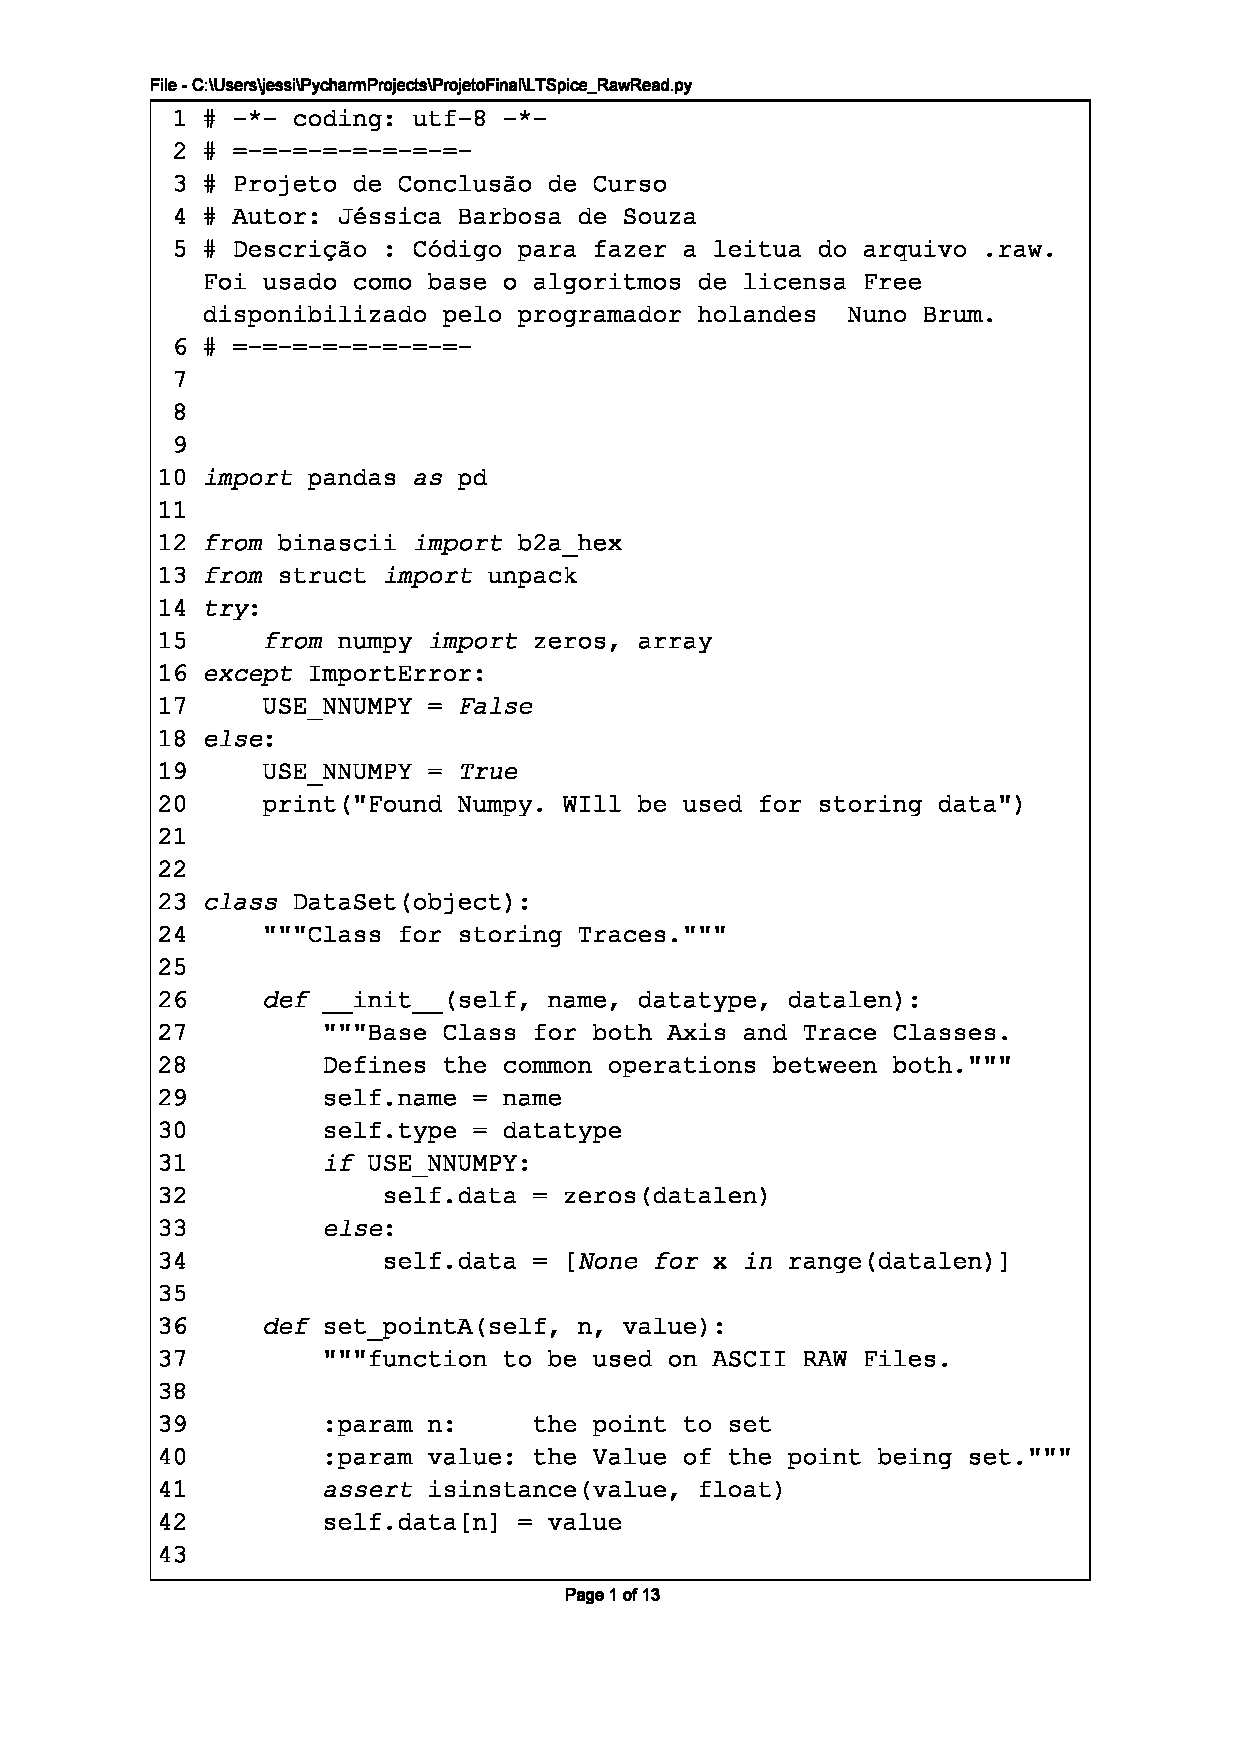
\includegraphics[scale=0.75]{01_Pre_textuais/code/leitura1.pdf}
\end{figure}
\newpage

\begin{figure}[H]
\centering
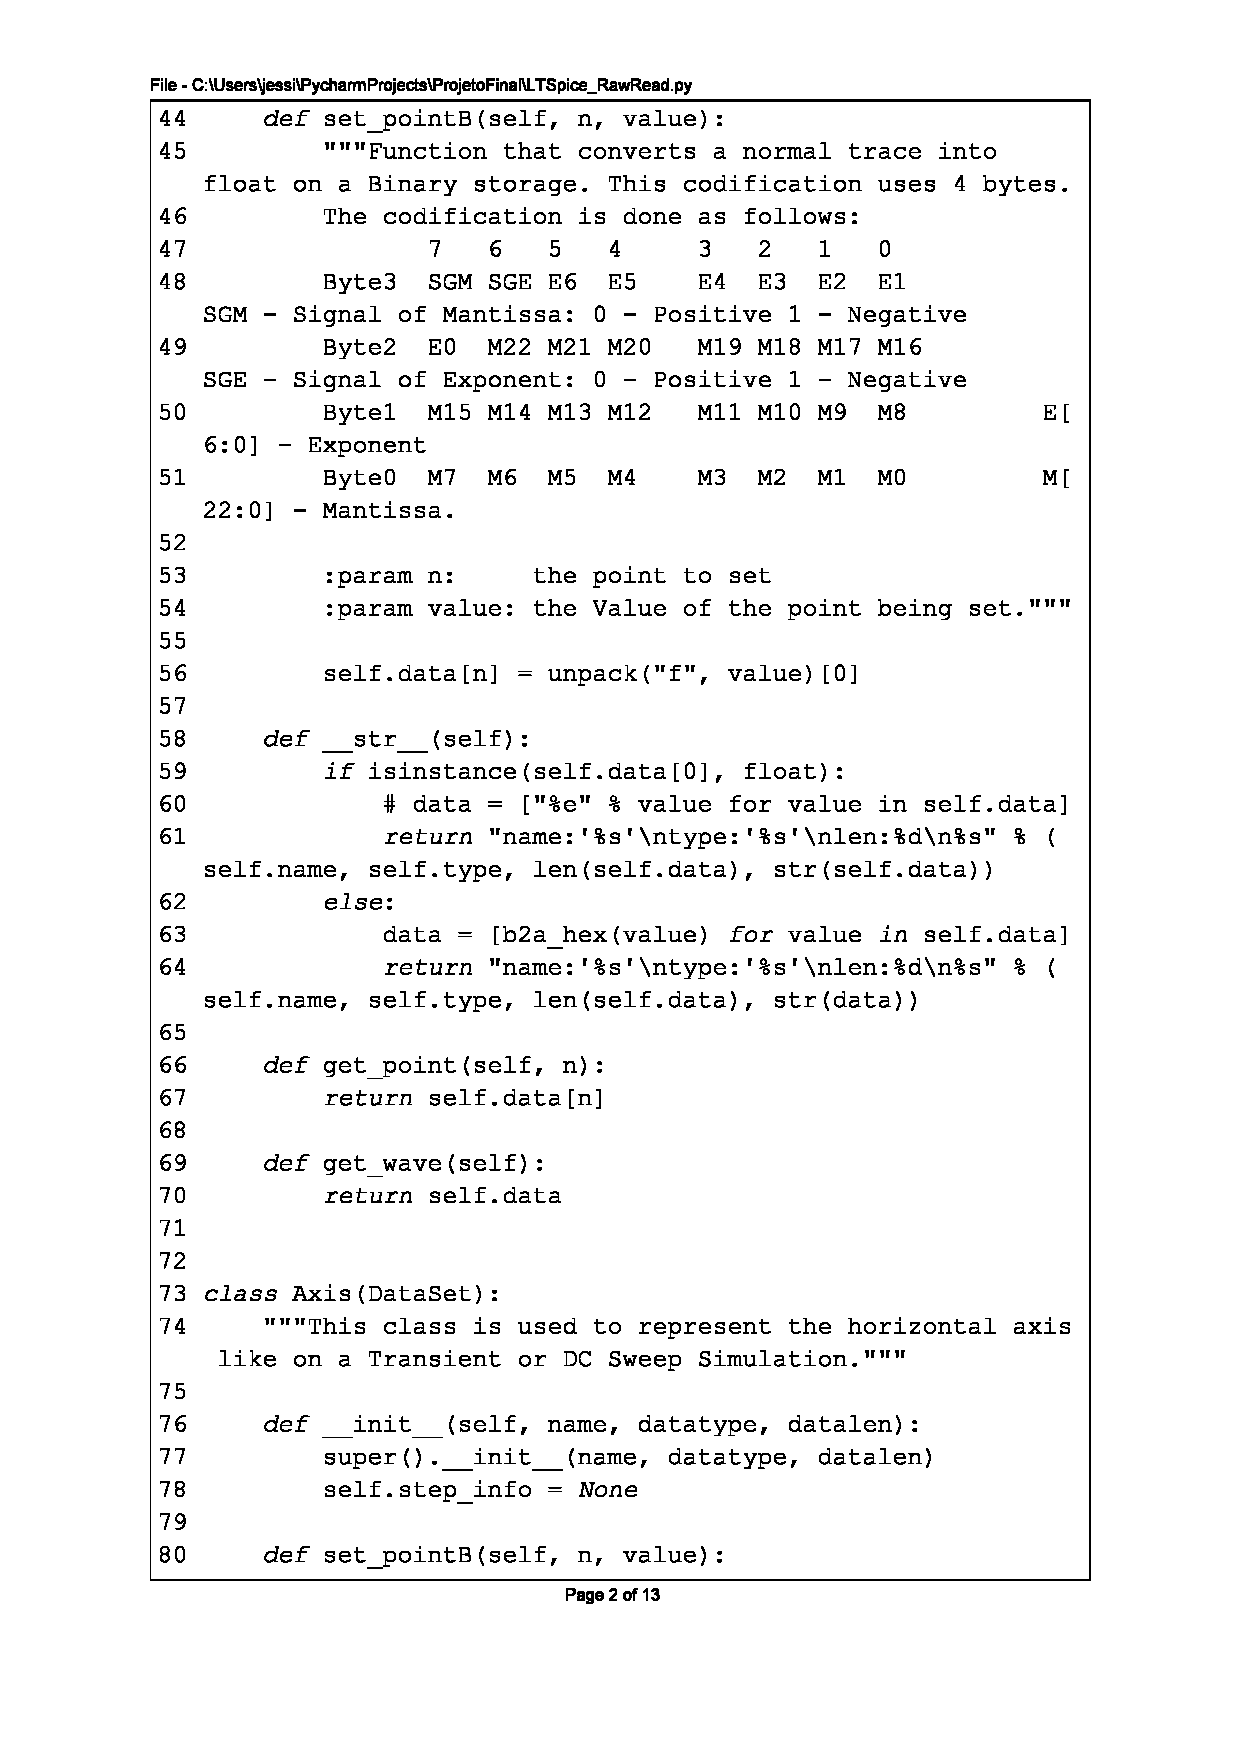
\includegraphics[scale=0.9]{01_Pre_textuais/code/leitura2.pdf}
\end{figure}


\begin{figure}[H]
\centering
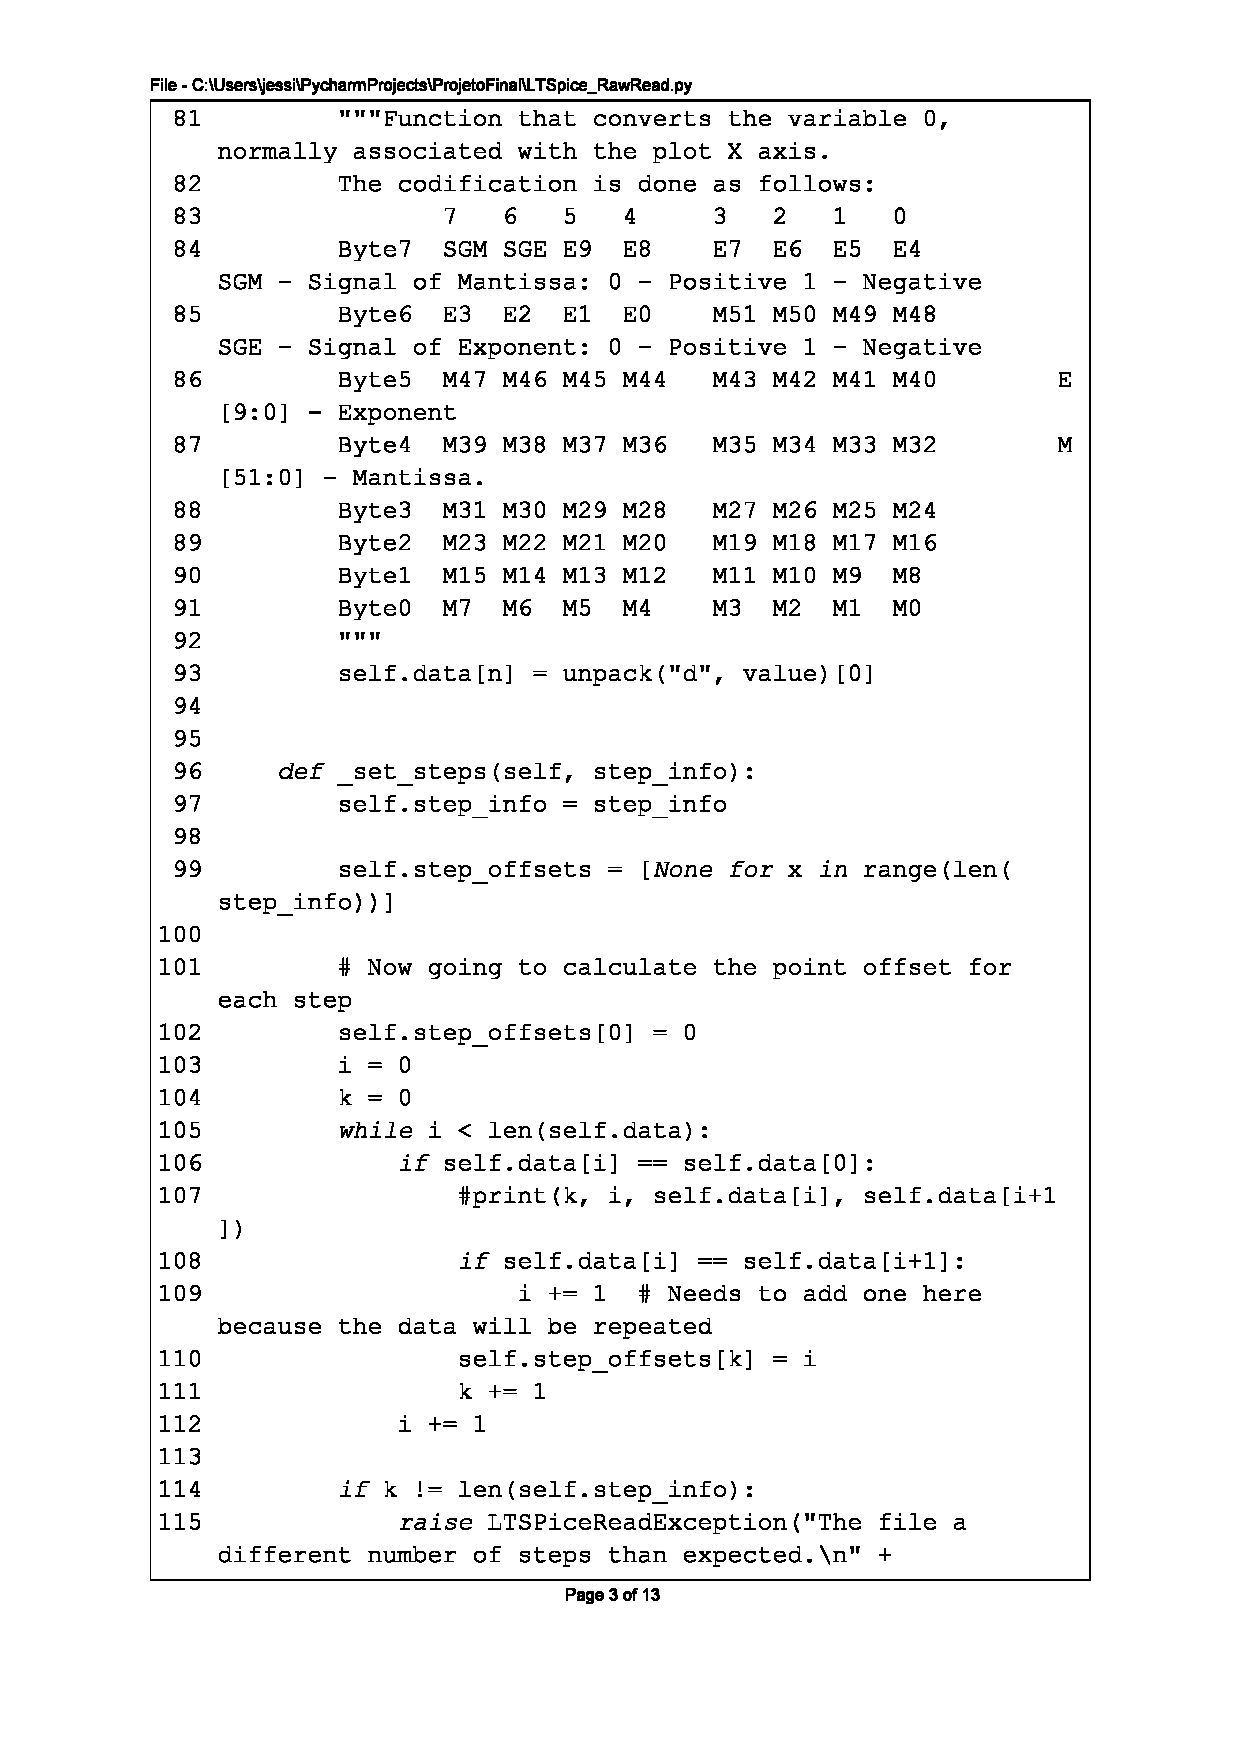
\includegraphics[scale=0.9]{01_Pre_textuais/code/leitura3.pdf}
\end{figure}
\begin{figure}[H]
\centering
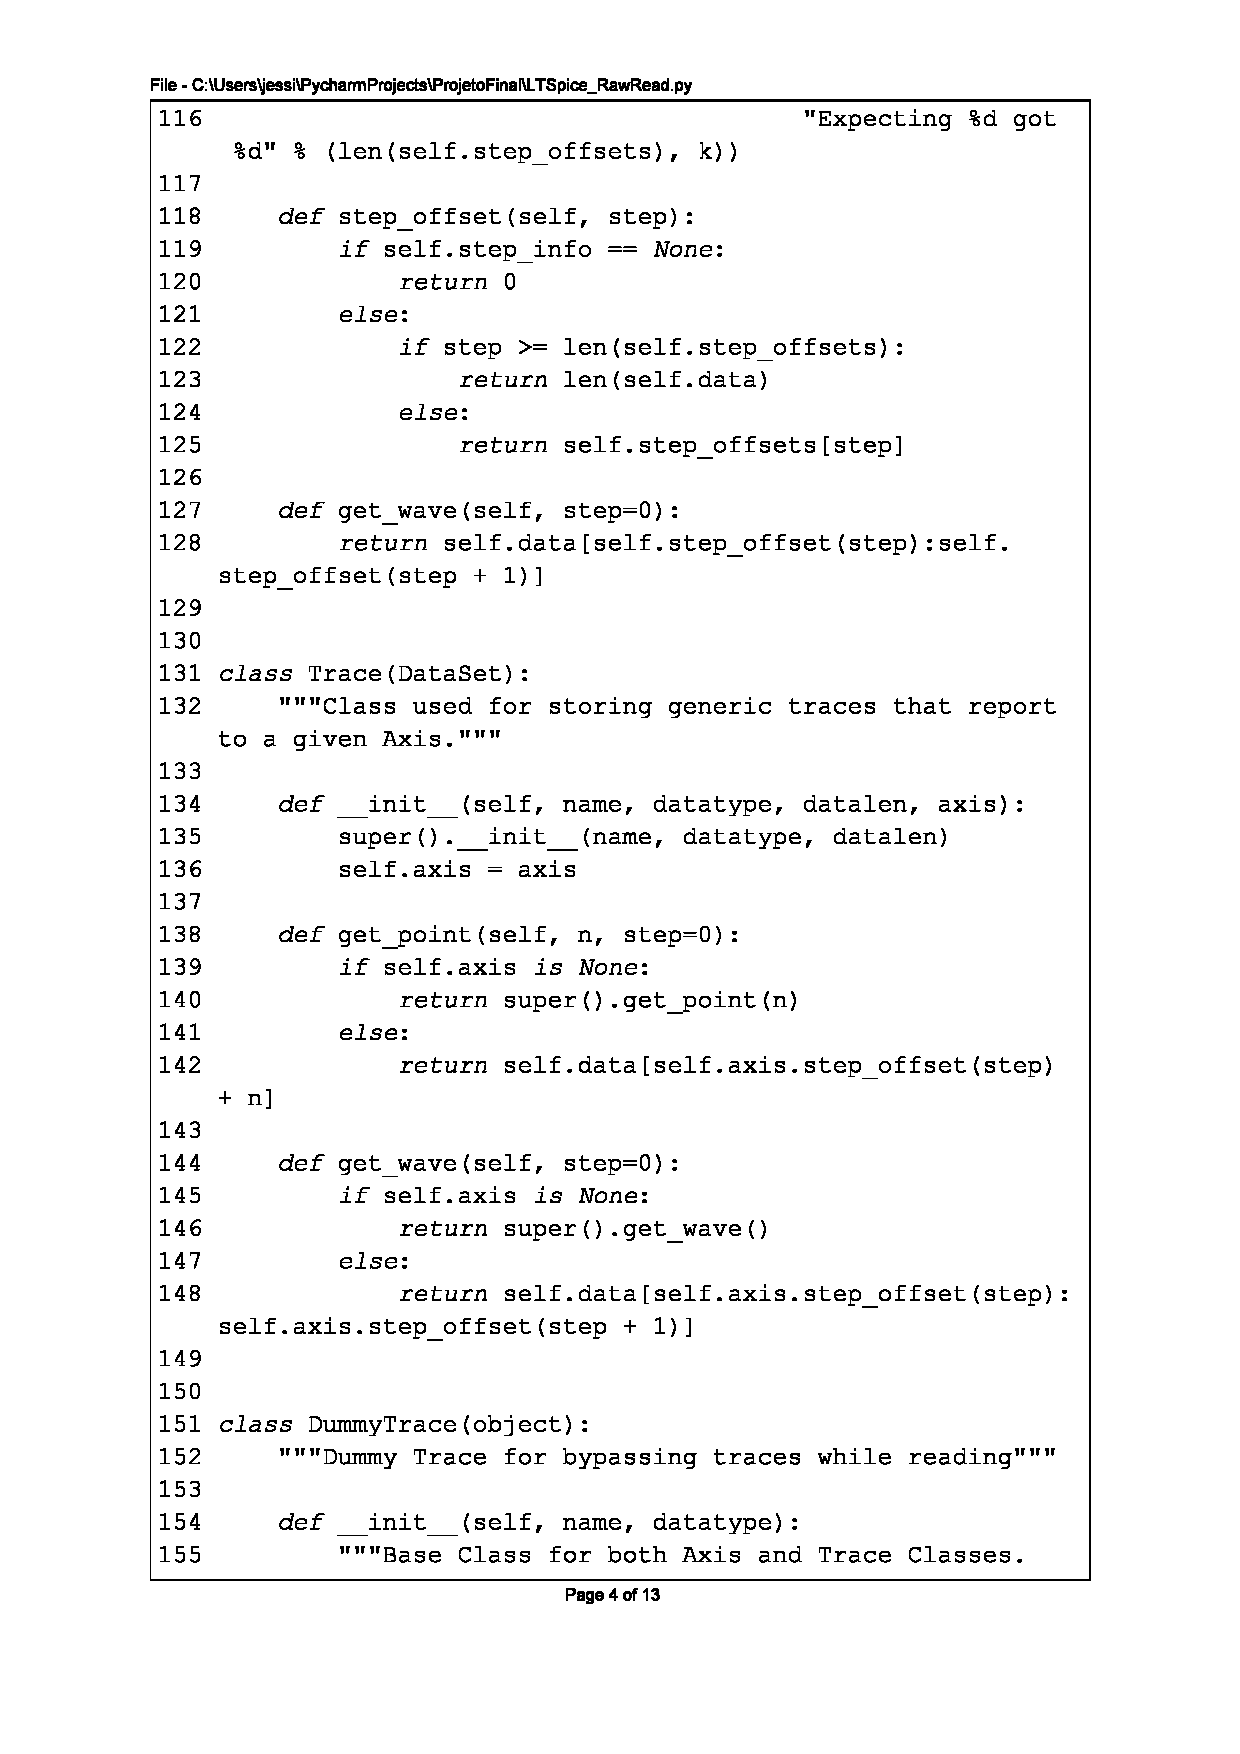
\includegraphics[scale=0.9]{01_Pre_textuais/code/leitura4.pdf}
\end{figure}
\begin{figure}[]
\centering
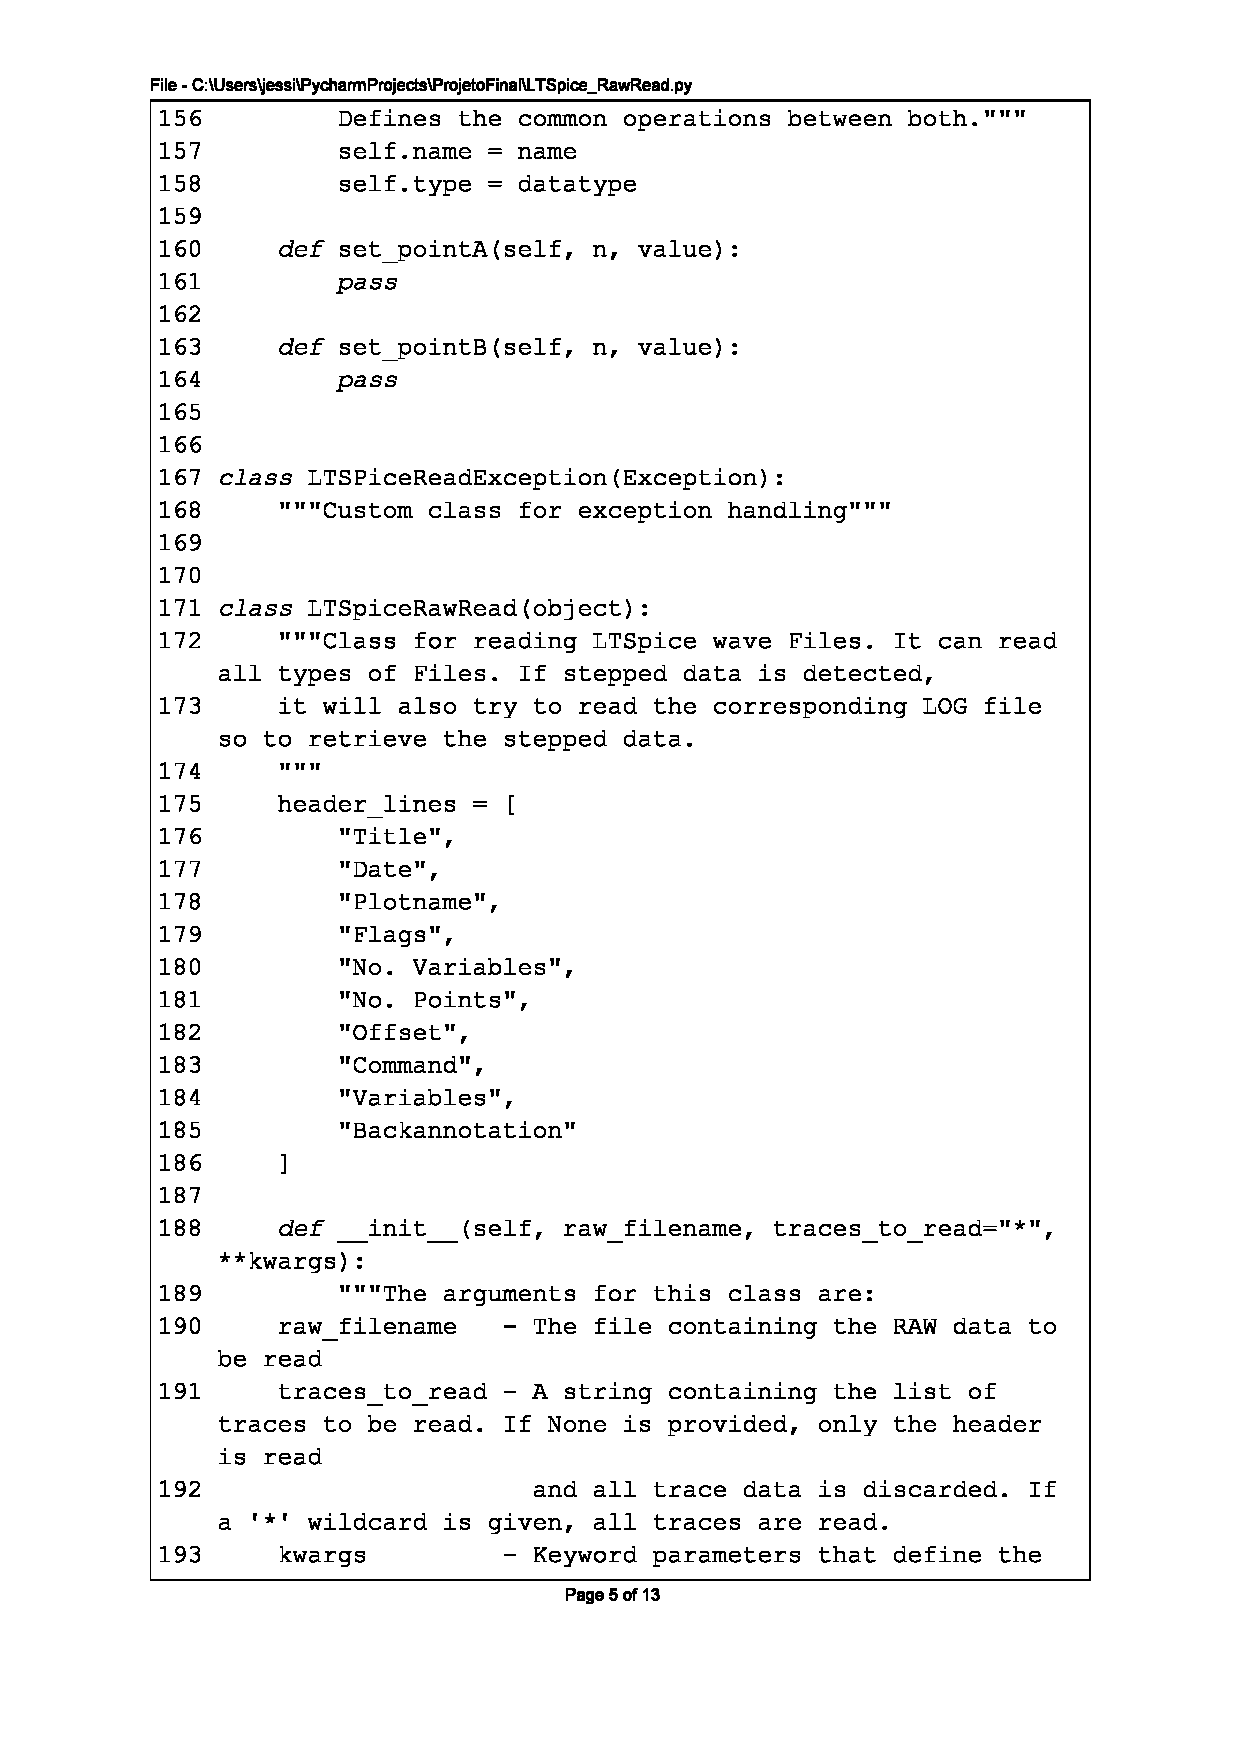
\includegraphics[scale=0.9]{01_Pre_textuais/code/leitura5.pdf}
\end{figure}
\begin{figure}[]
\centering
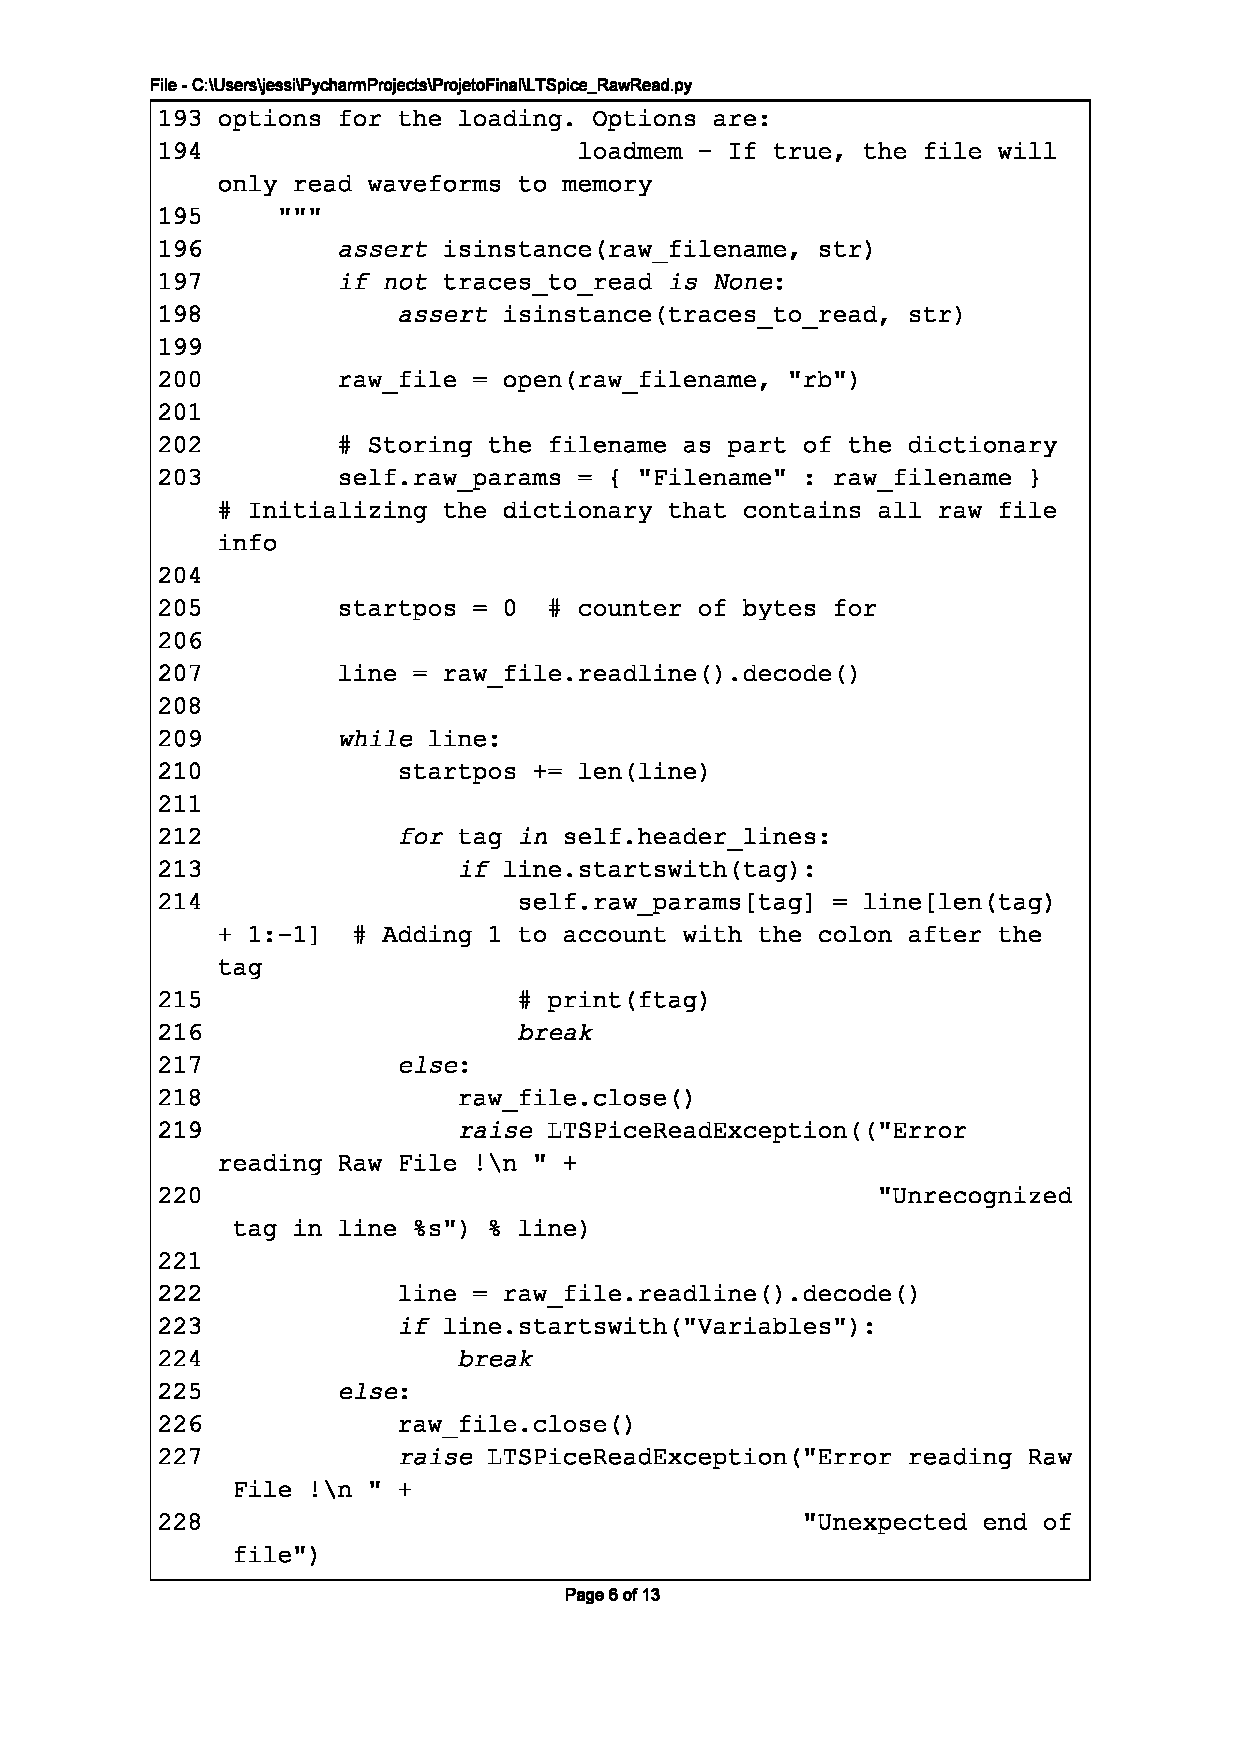
\includegraphics[scale=0.9]{01_Pre_textuais/code/leitura6.pdf}
\end{figure}
\begin{figure}[]
\centering
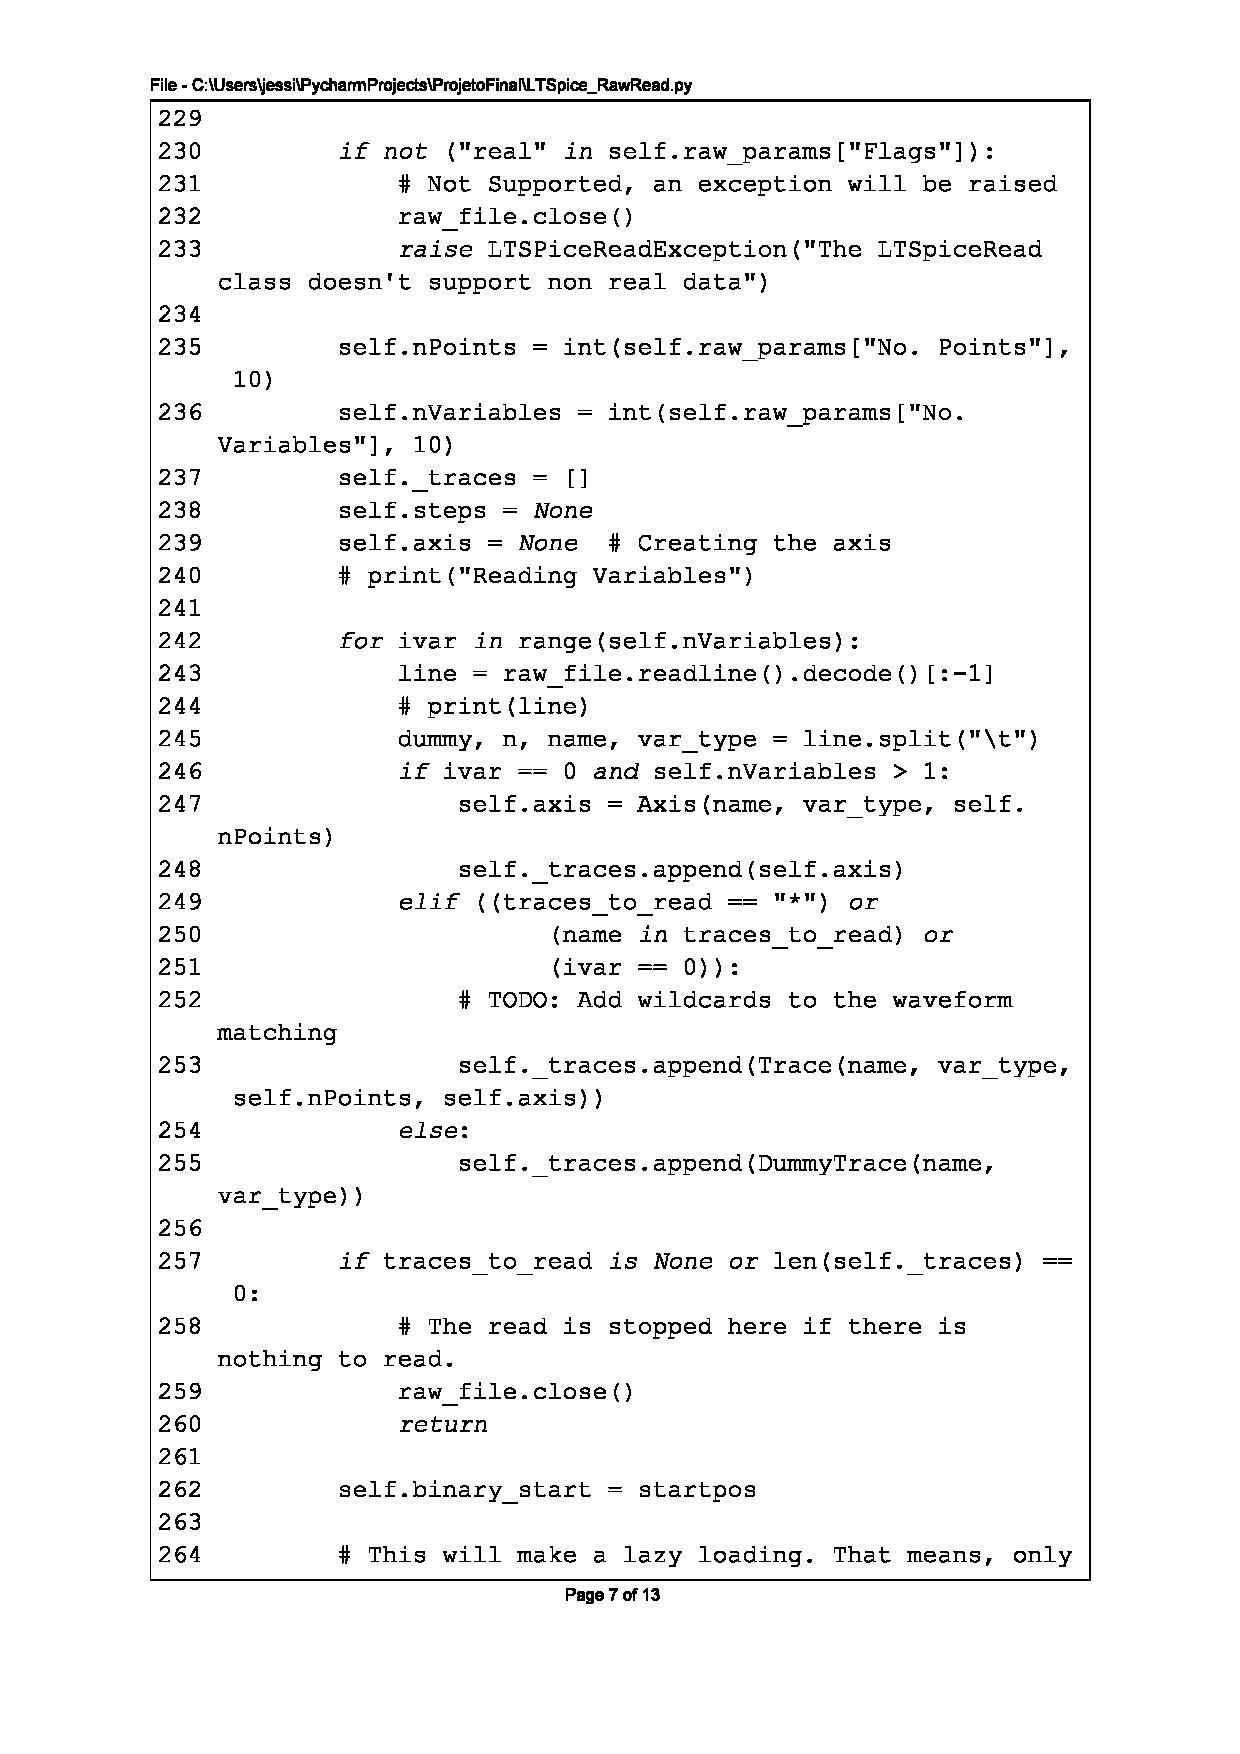
\includegraphics[scale=0.9]{01_Pre_textuais/code/leitura7.pdf}
\end{figure}
\begin{figure}[]
\centering
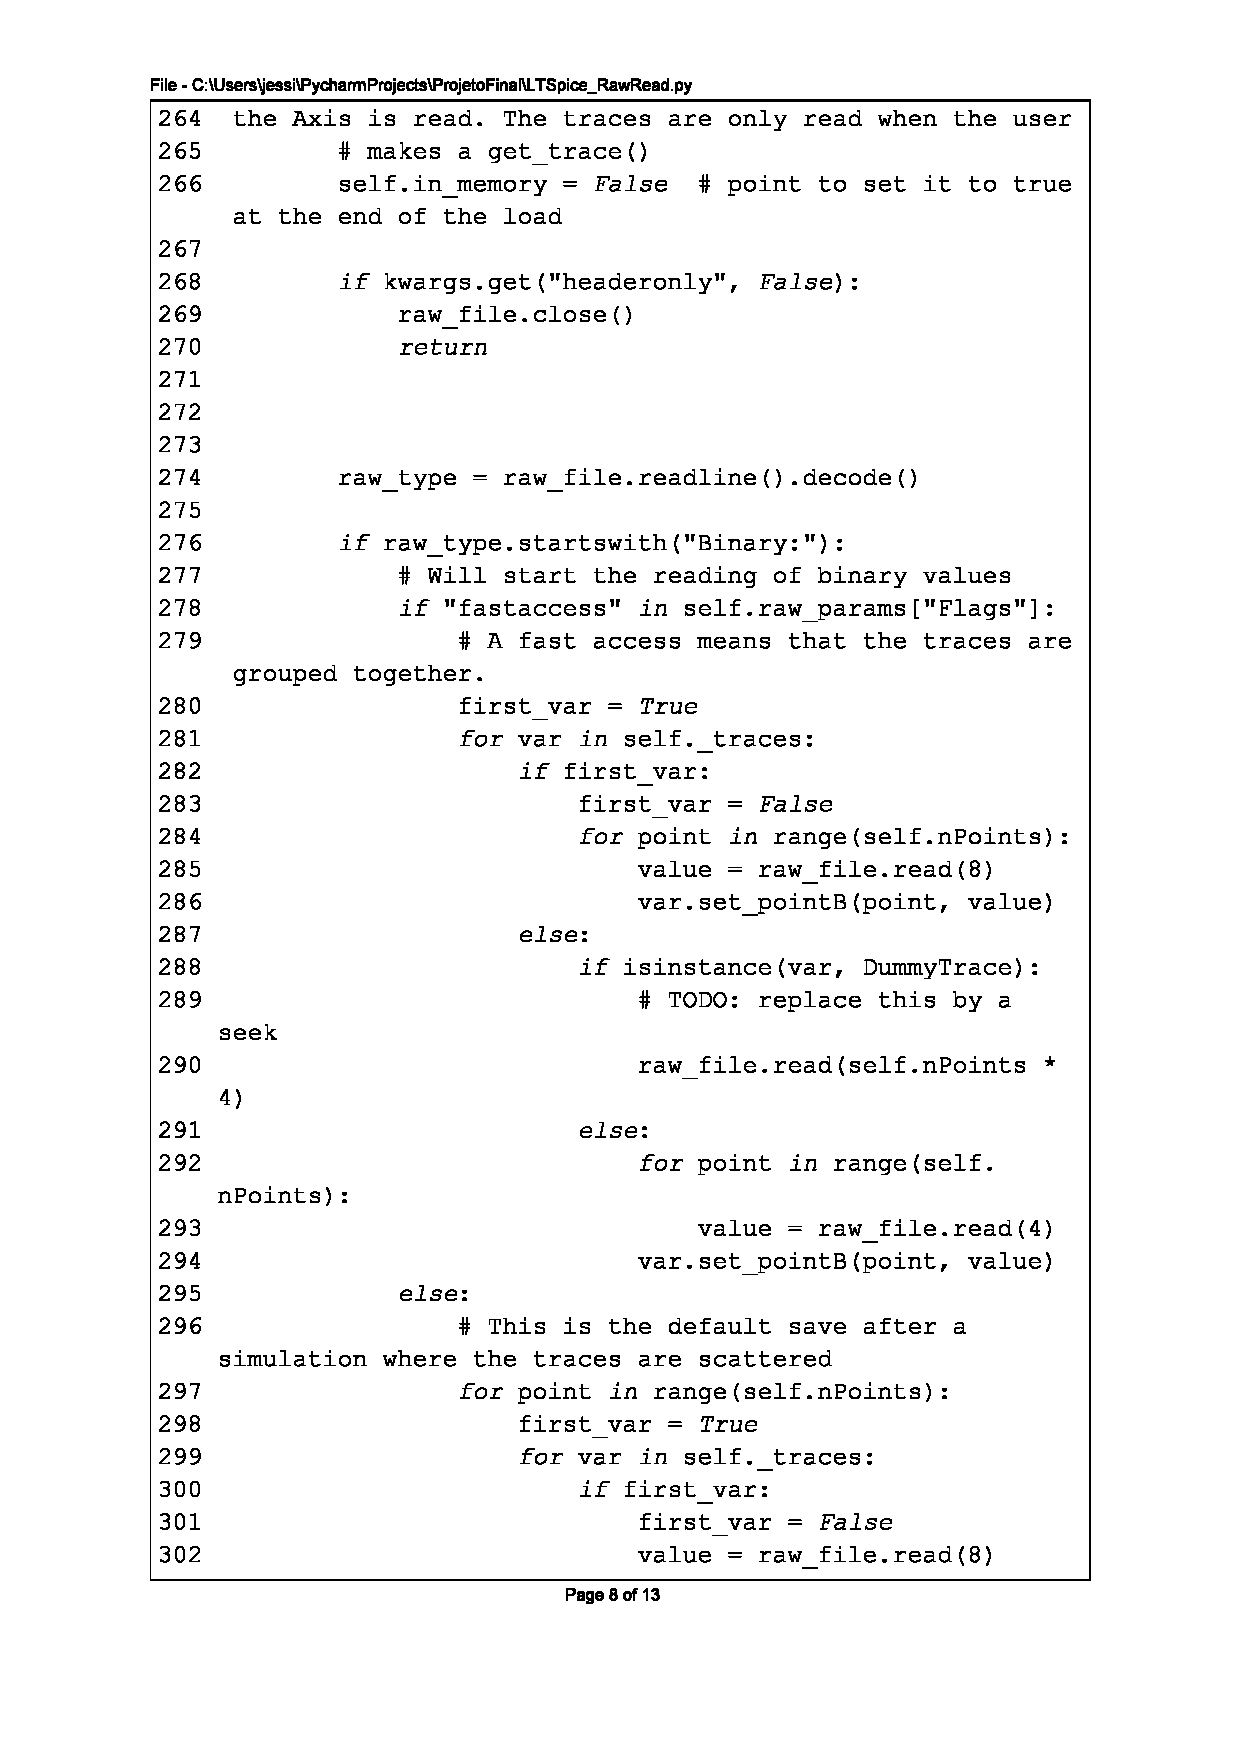
\includegraphics[scale=0.9]{01_Pre_textuais/code/leitura8.pdf}
\end{figure}
\begin{figure}[]
\centering
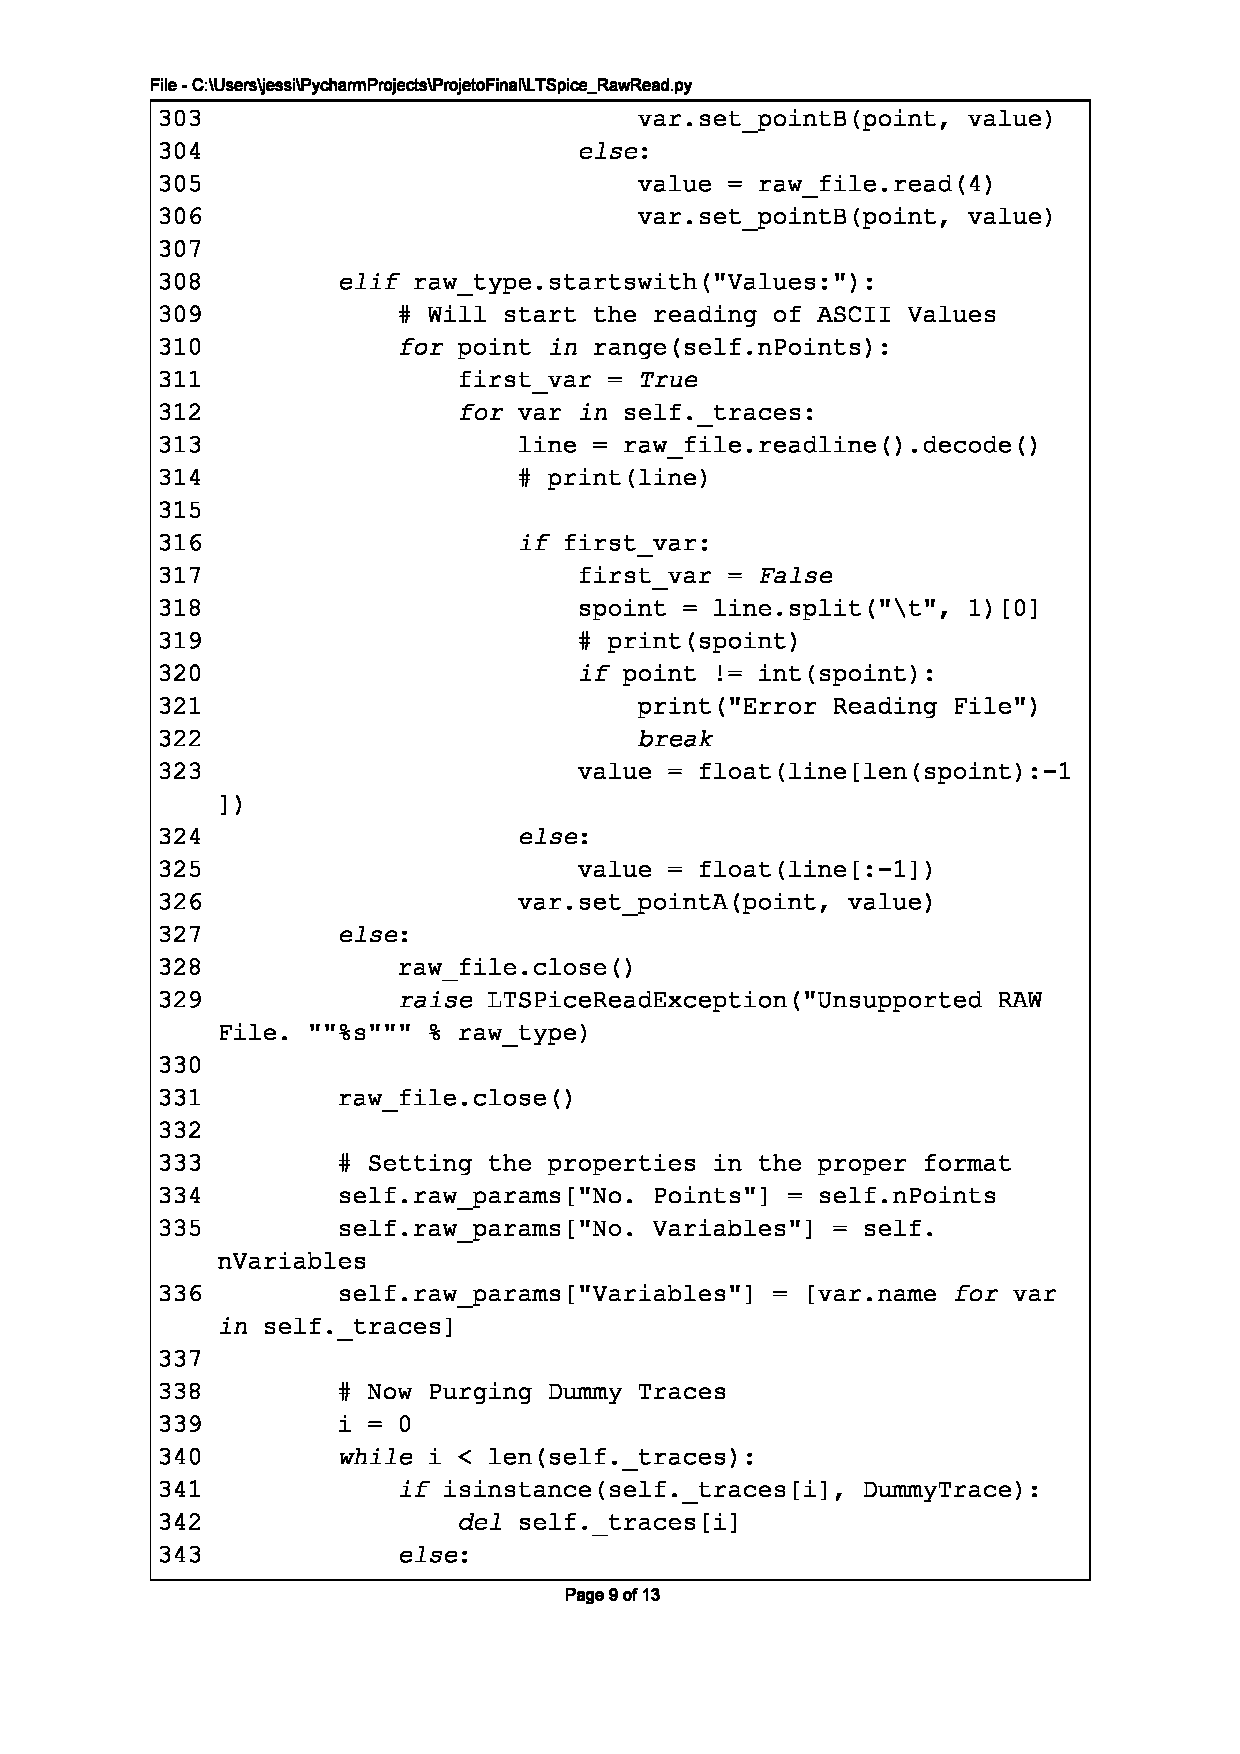
\includegraphics[scale=0.9]{01_Pre_textuais/code/leitura9.pdf}
\end{figure}
\begin{figure}[]
\centering
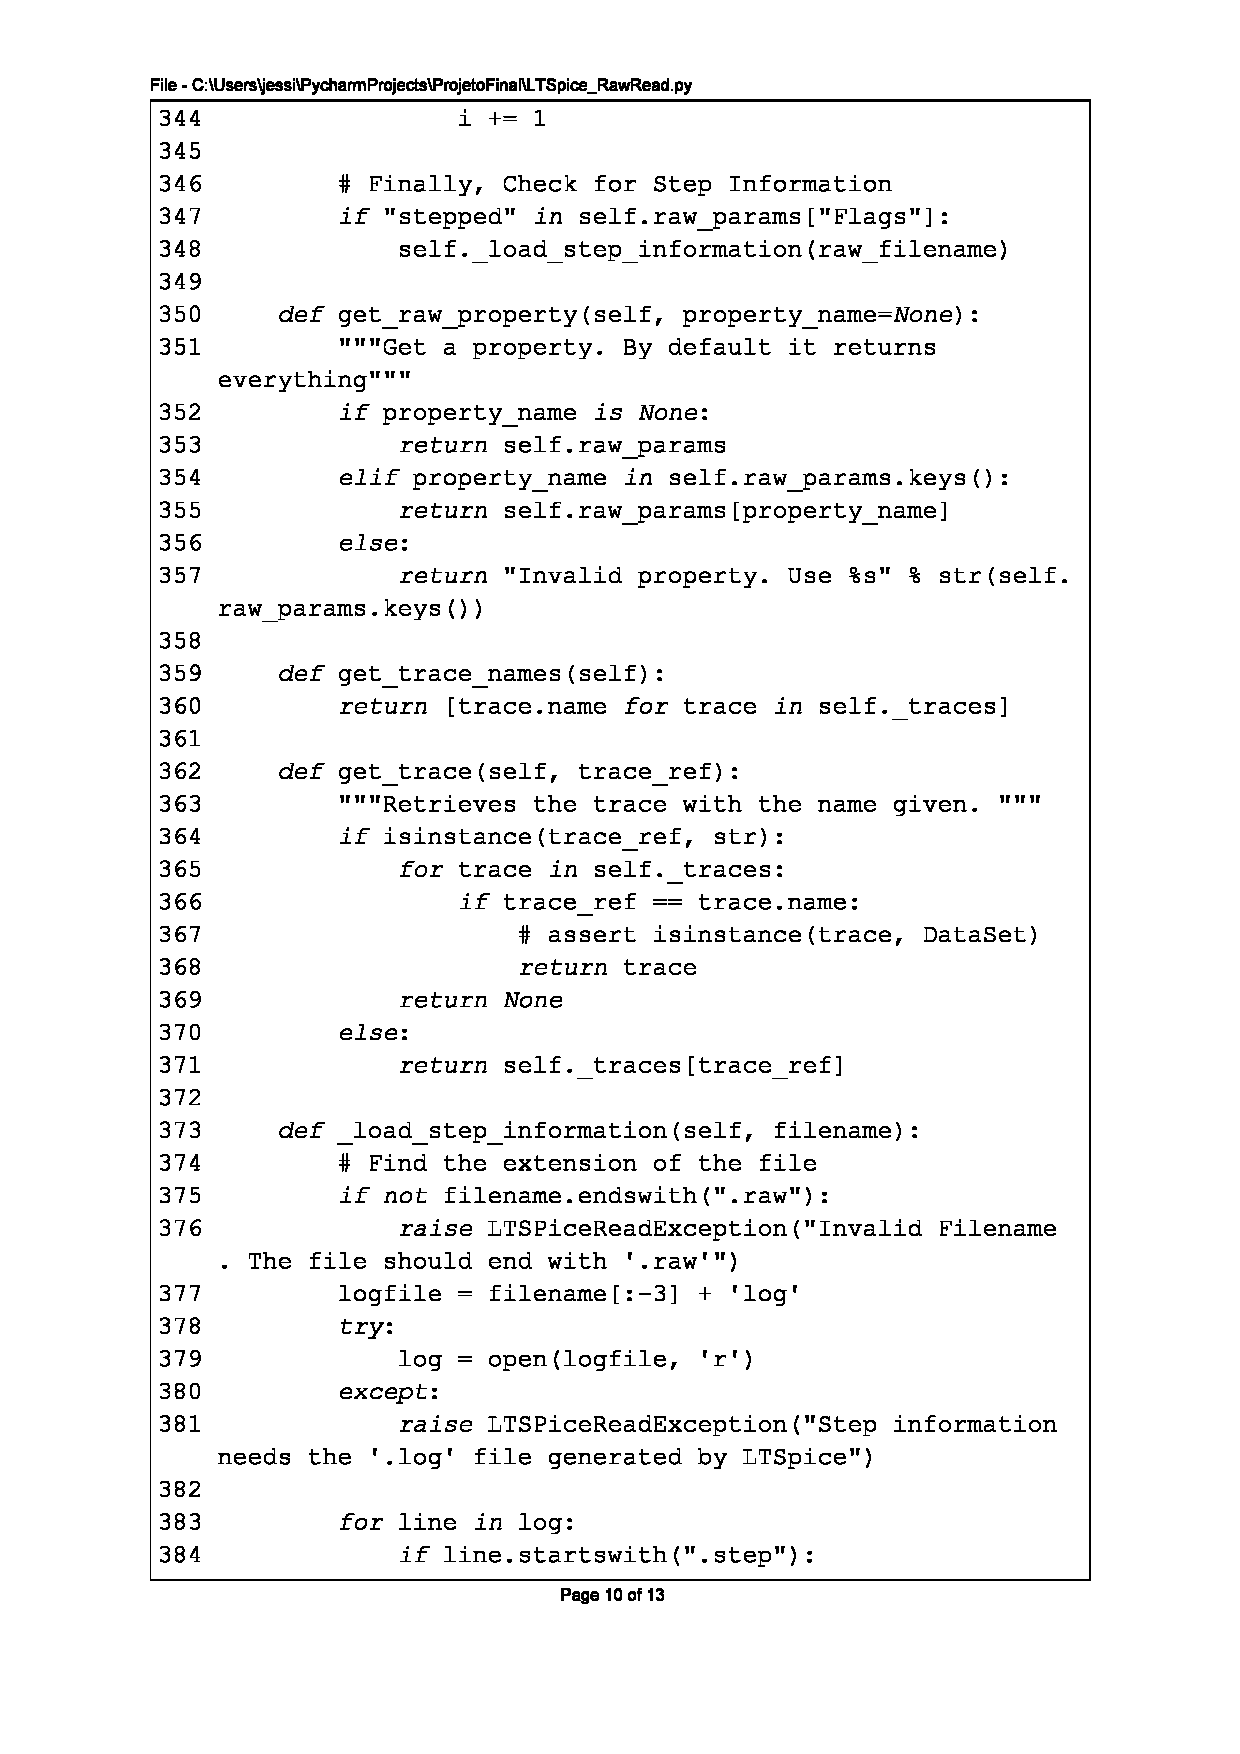
\includegraphics[scale=0.9]{01_Pre_textuais/code/leitura10.pdf}
\end{figure}

\begin{figure}[]
\centering
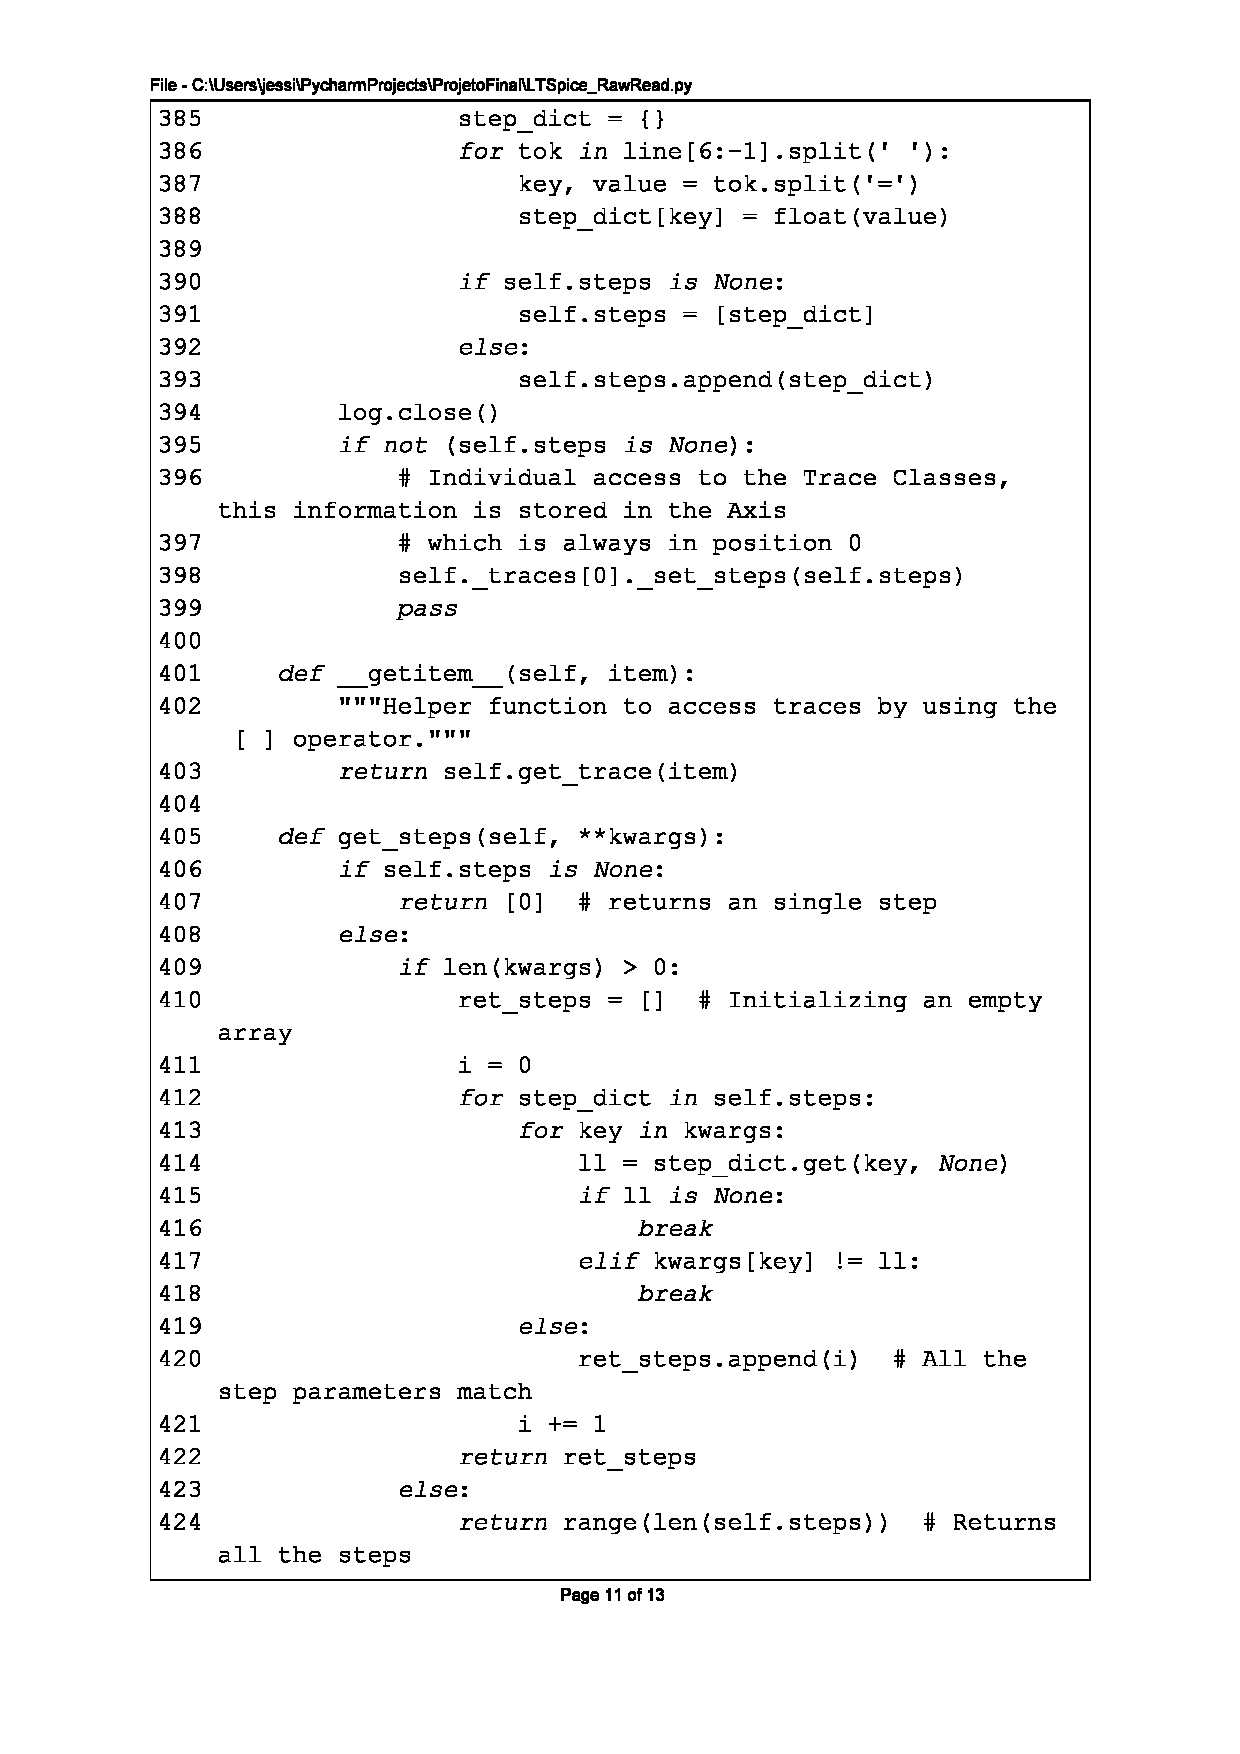
\includegraphics[scale=0.9]{01_Pre_textuais/code/leitura11.pdf}
\end{figure}

\begin{figure}[]
\centering
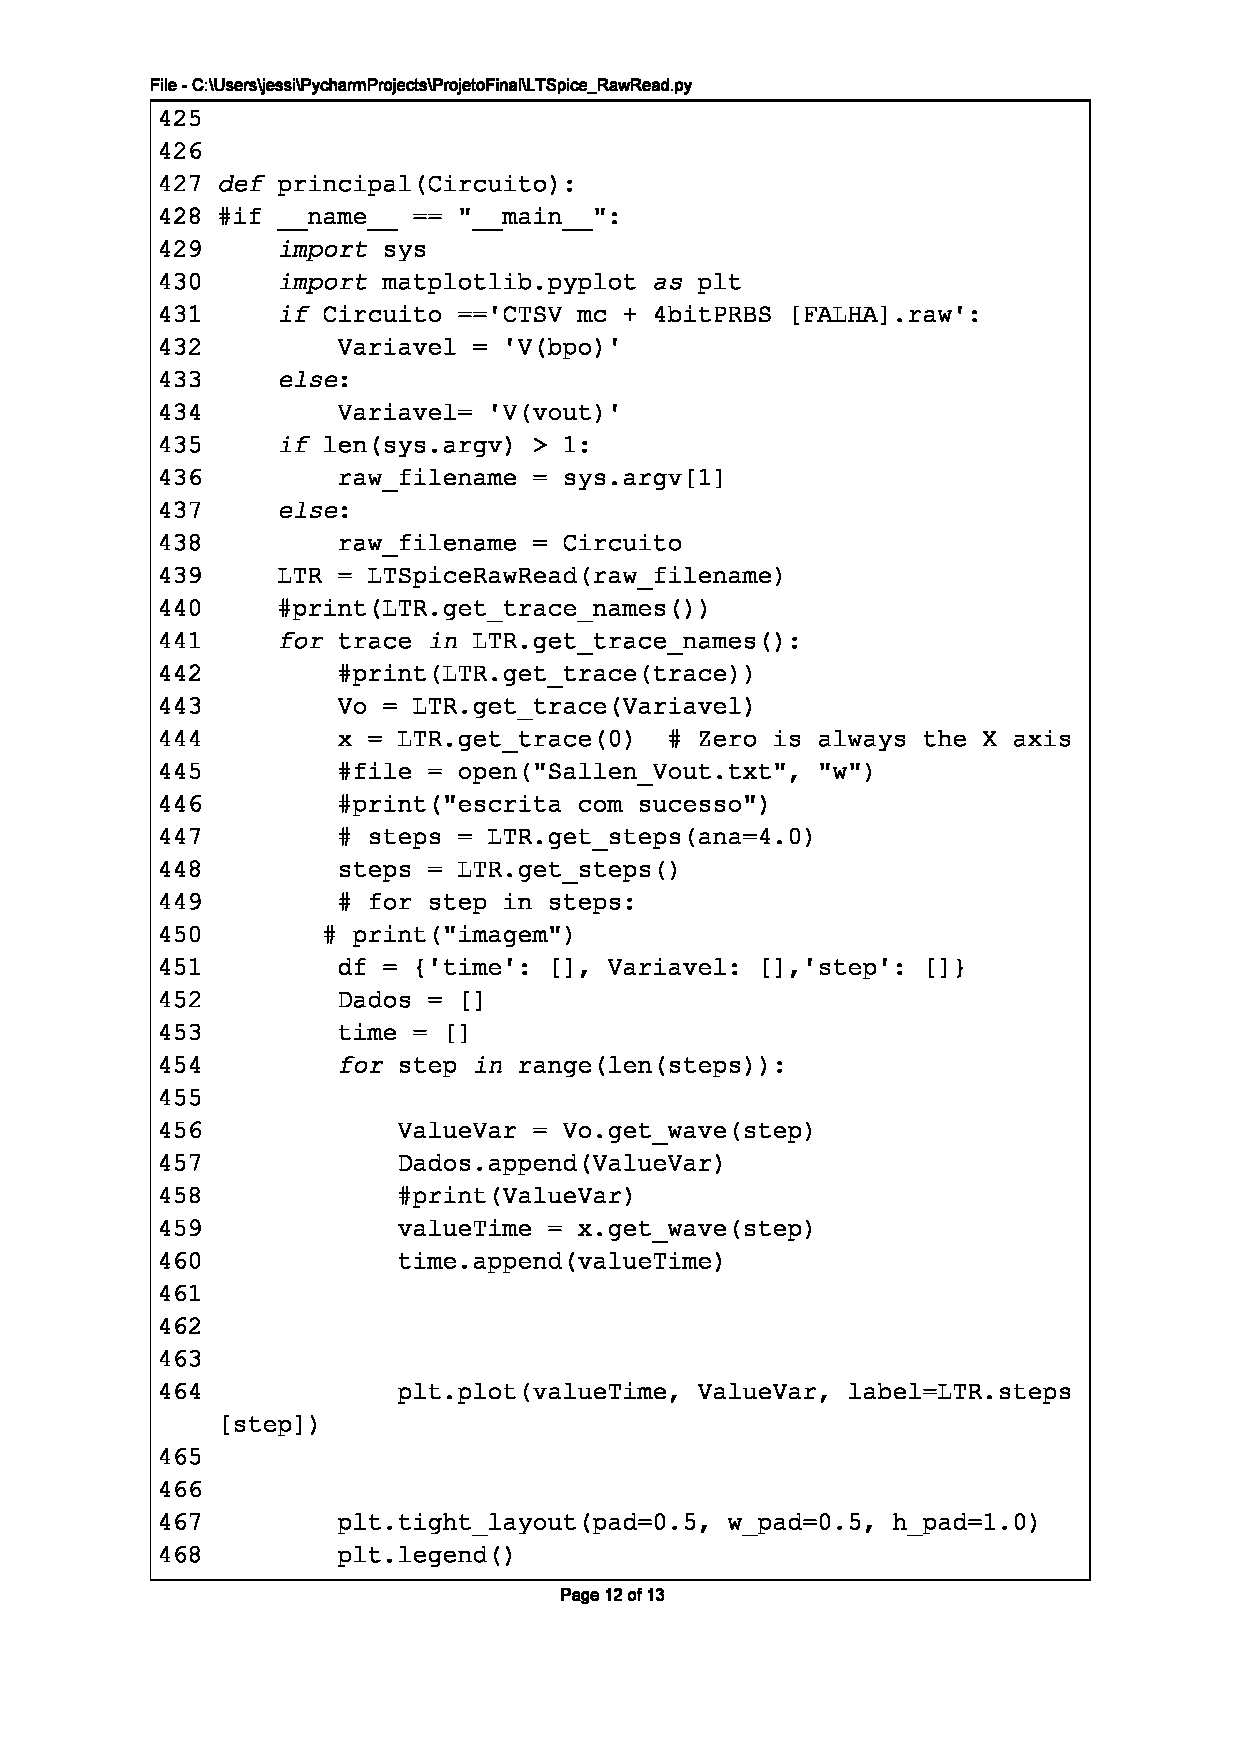
\includegraphics[scale=0.9]{01_Pre_textuais/code/leitura12.pdf}
\end{figure}
\begin{figure}[]
\centering
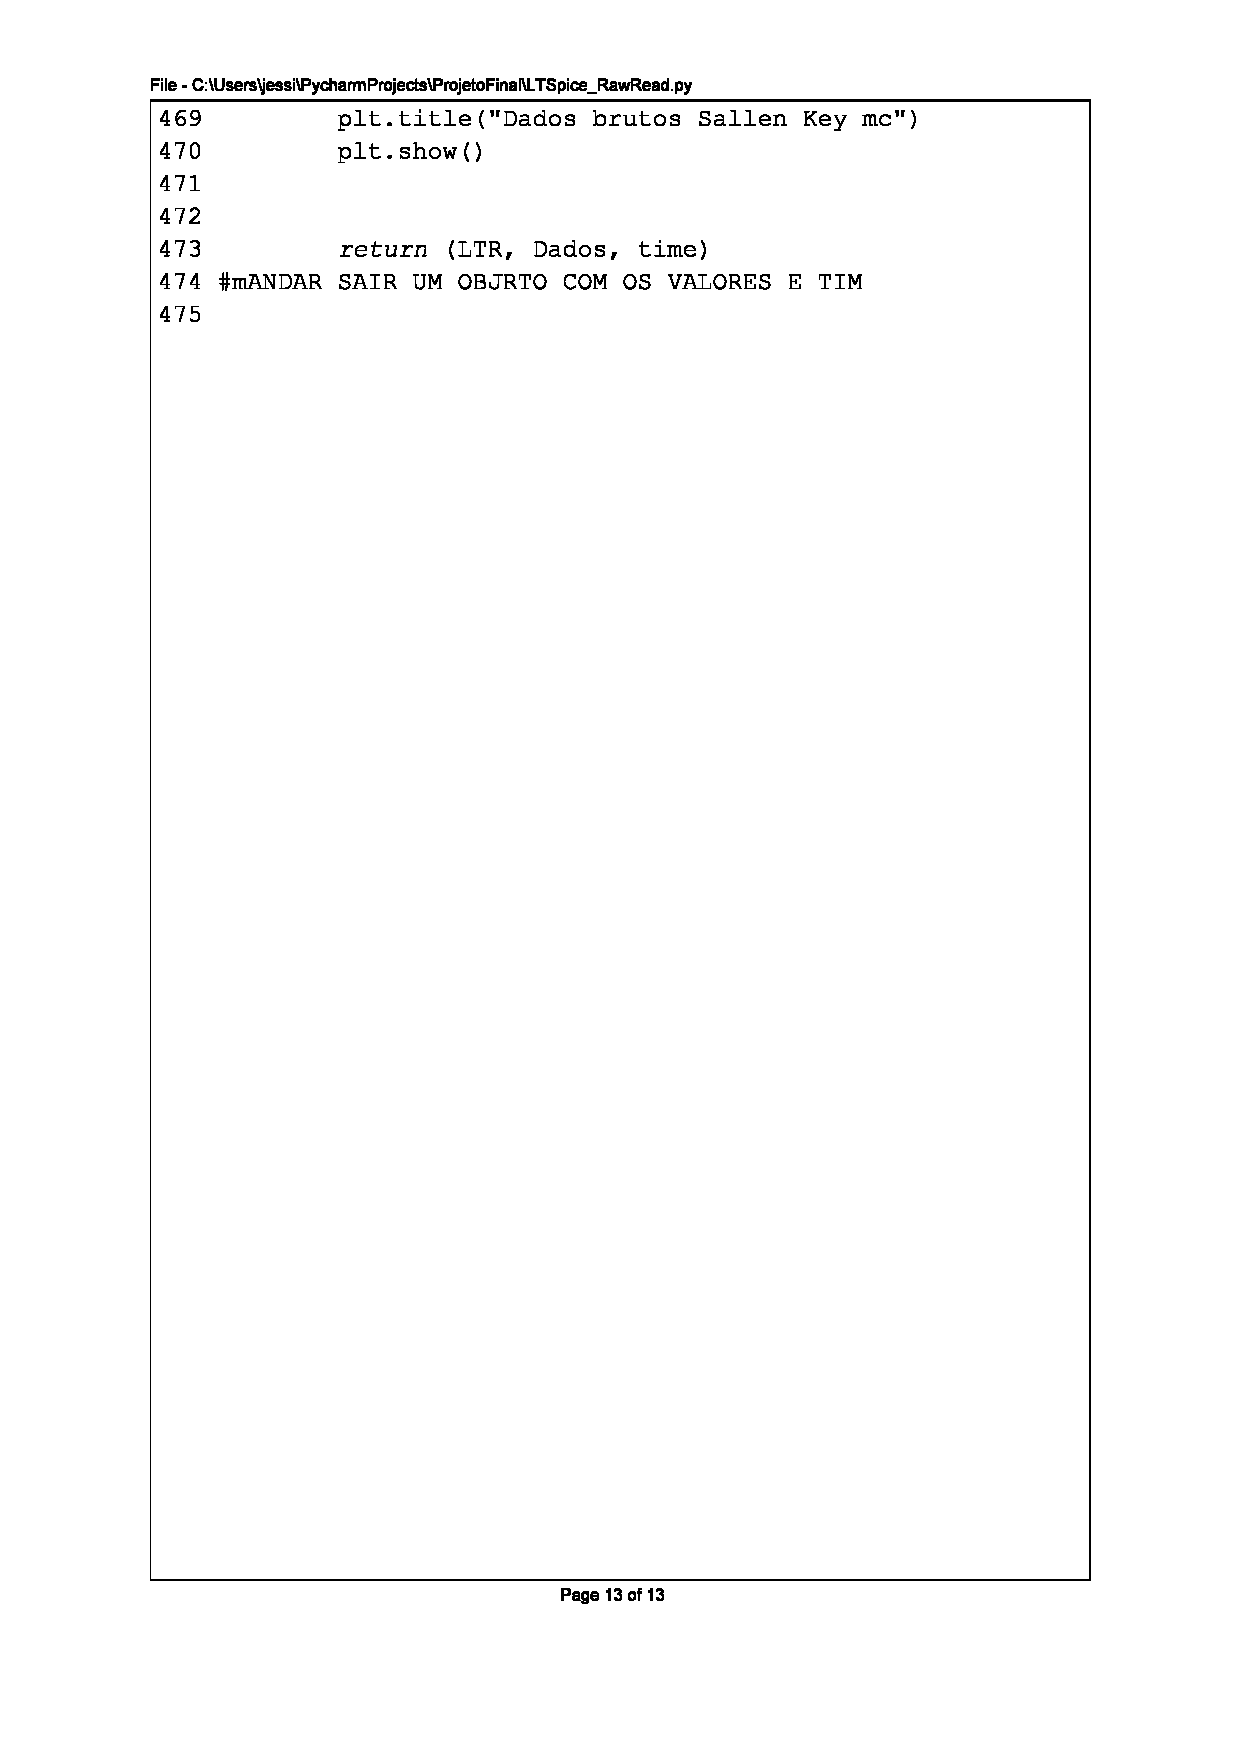
\includegraphics[scale=0.9]{01_Pre_textuais/code/leitura13.pdf}
\end{figure}

\newpage
\begin{itemize}
    \item Criação do Arquivo CSV \textit{.raw}
\end{itemize}

\begin{figure}[H]
\centering
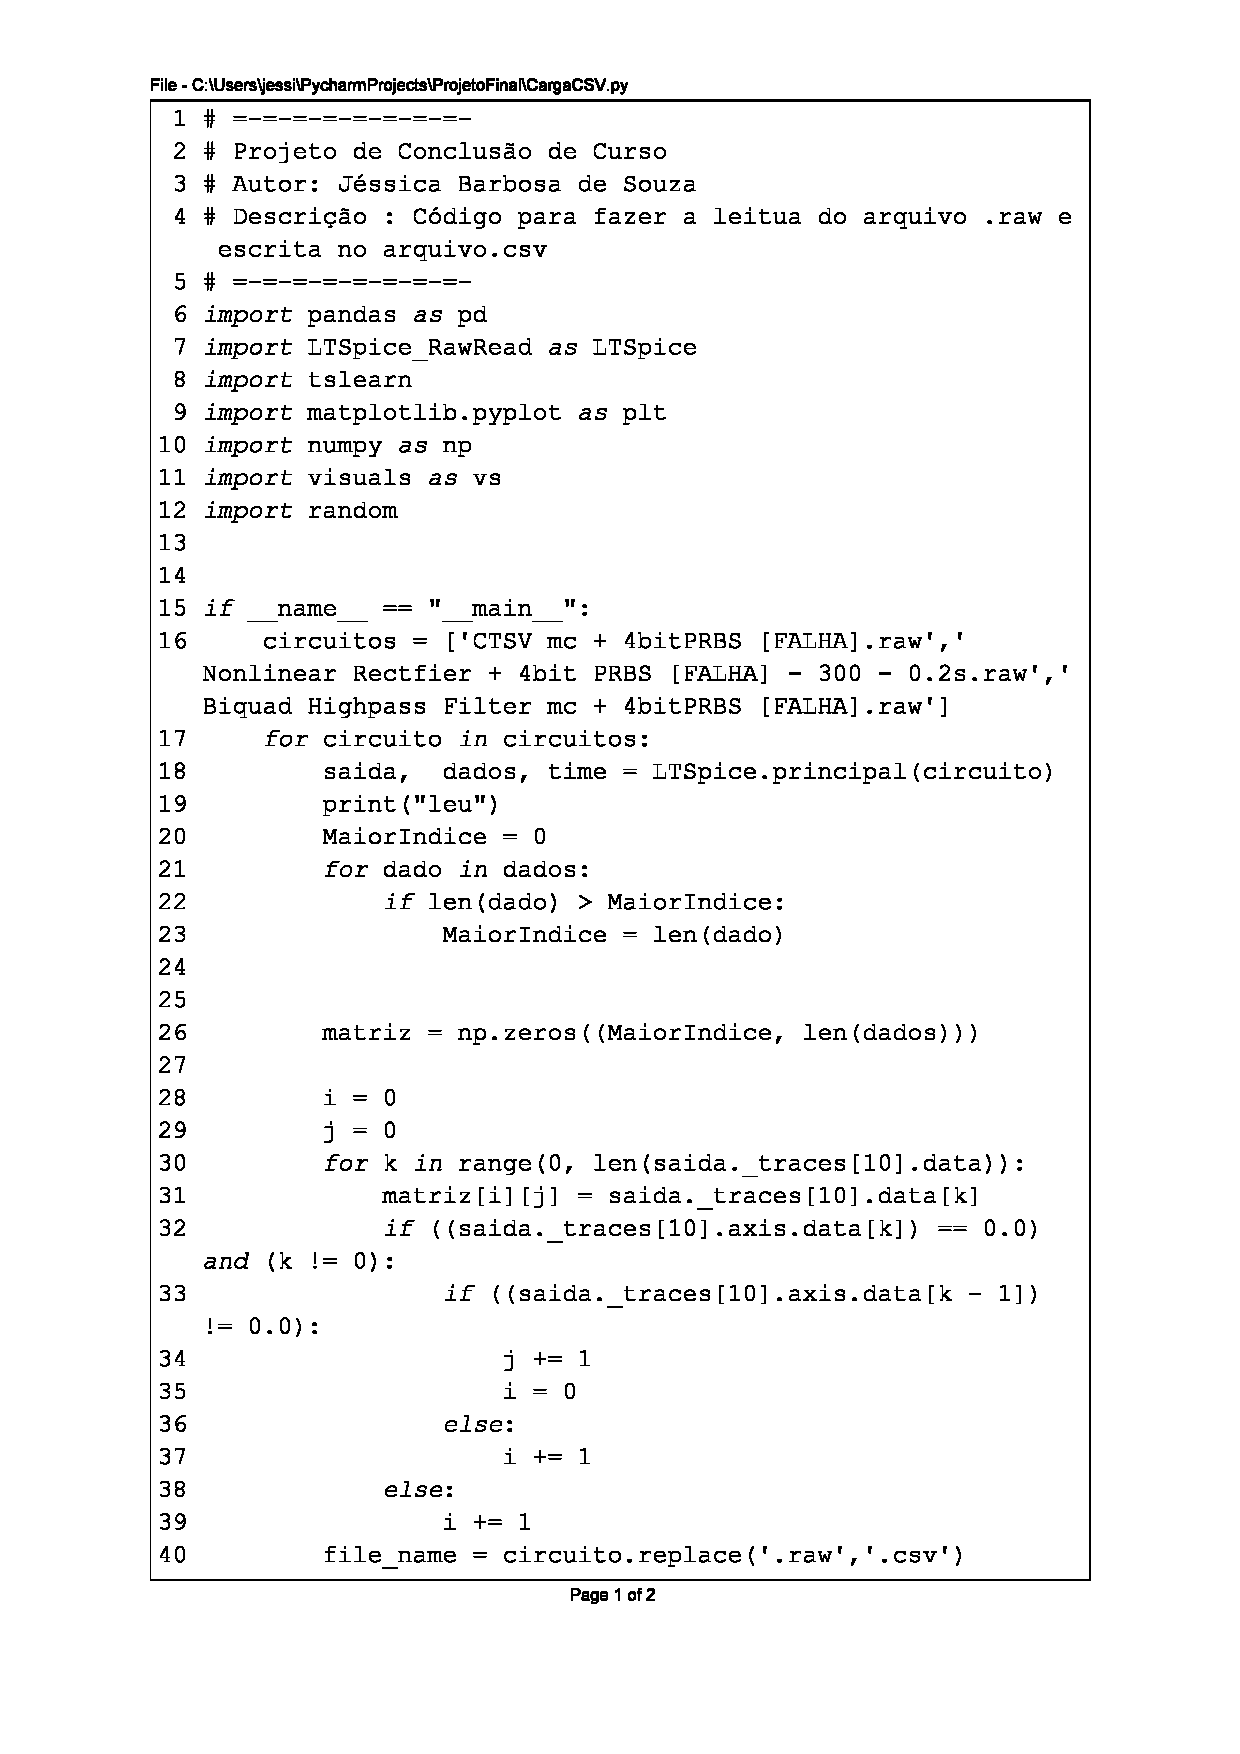
\includegraphics[scale=0.75]{01_Pre_textuais/code/CargaCsv.pdf}
\end{figure}

\newpage

\begin{itemize}
    \item Função com os algoritmos implementados
\end{itemize}
\begin{figure}[H]
\centering
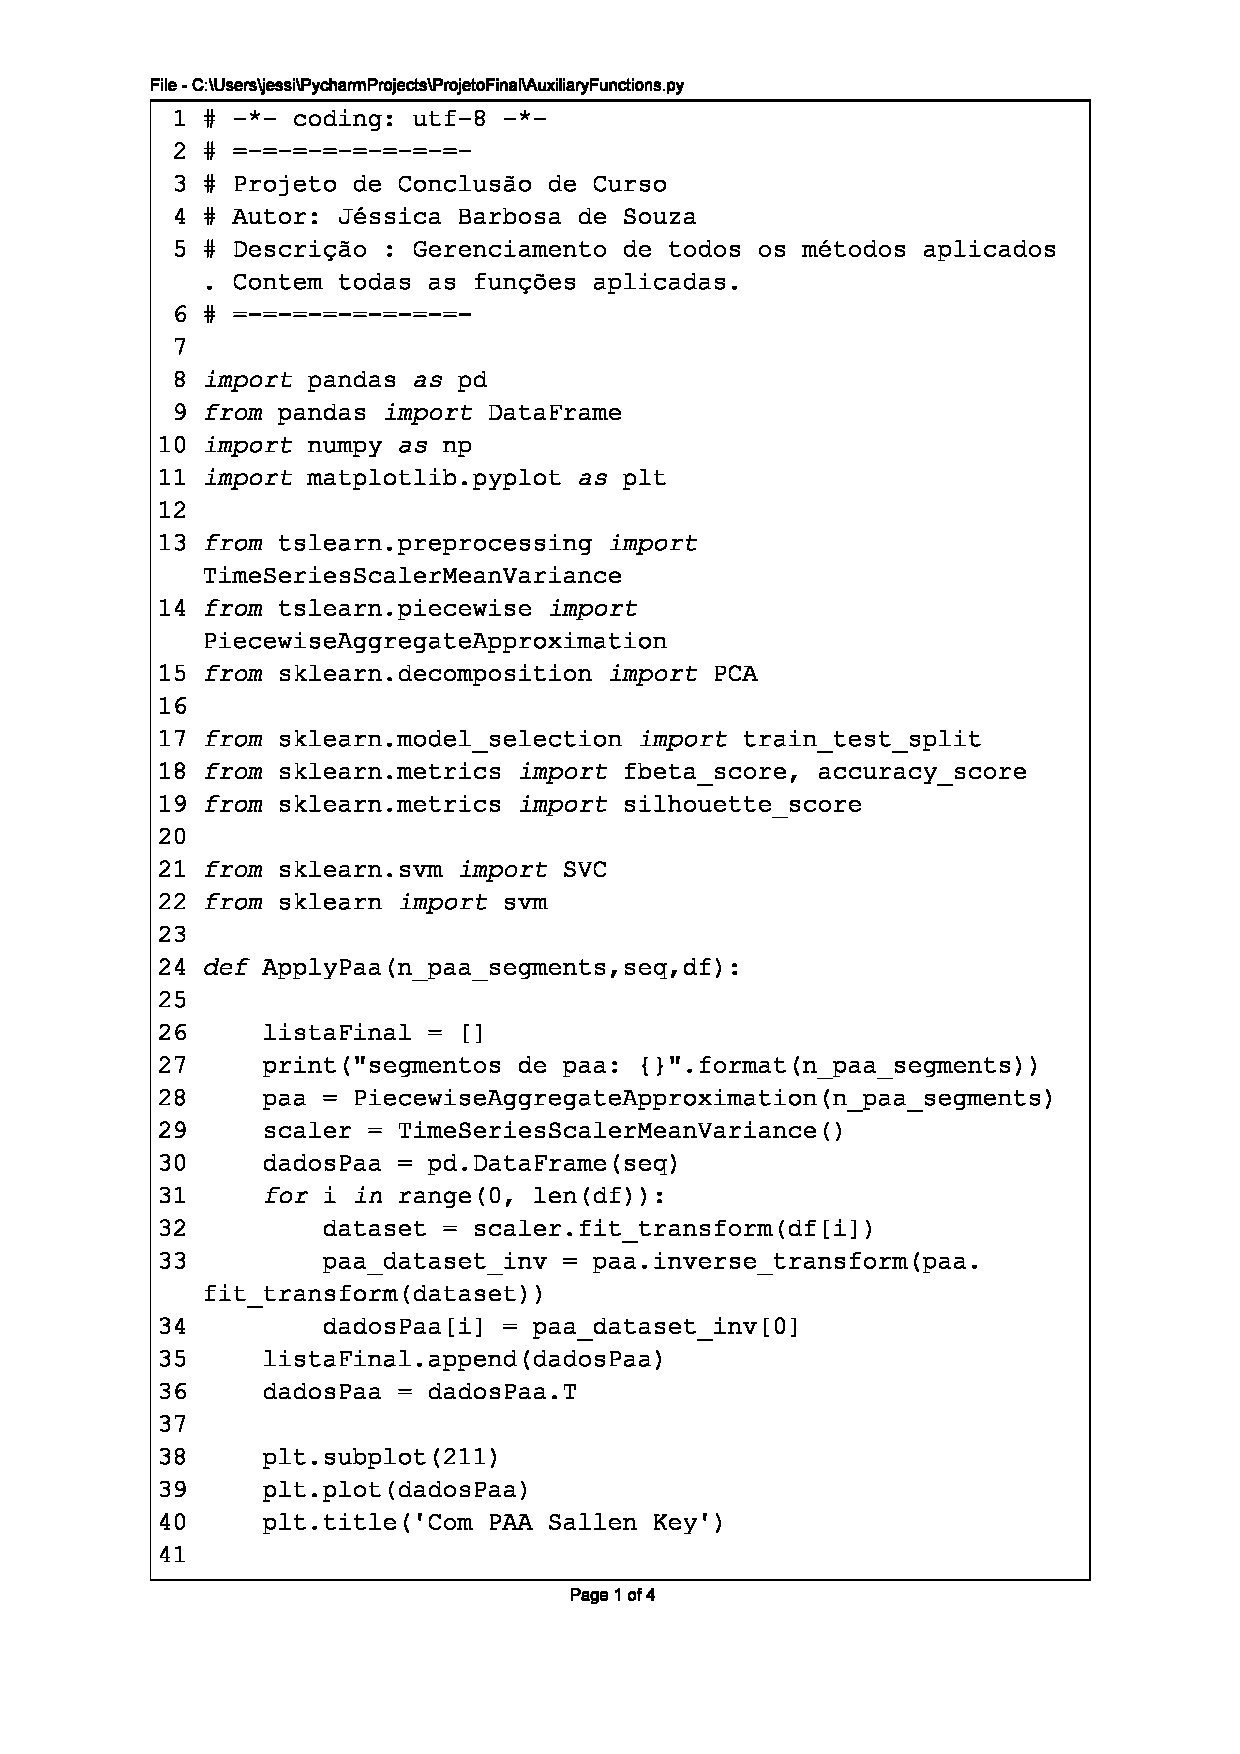
\includegraphics[scale=0.75]{01_Pre_textuais/code/analisa1.pdf}
\end{figure}

\begin{figure}[H]
\centering
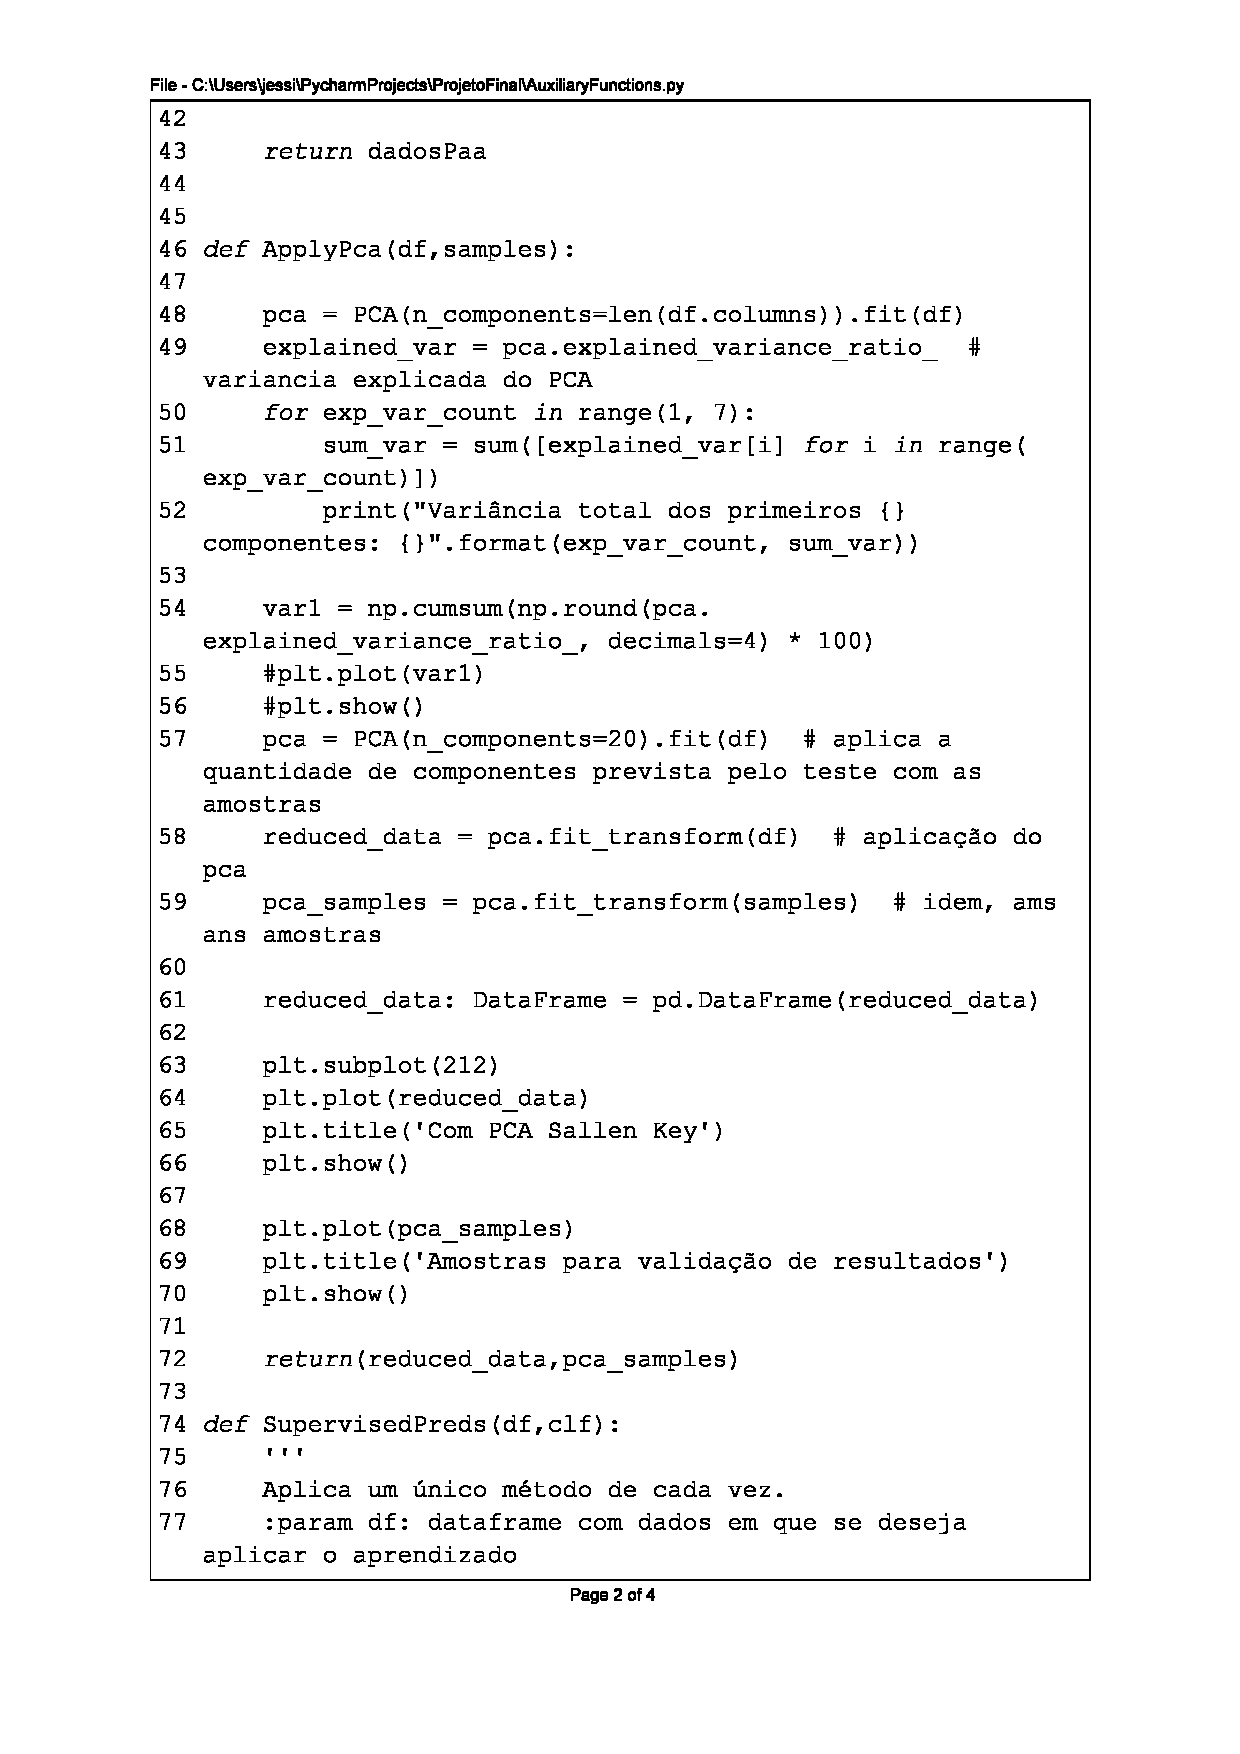
\includegraphics[scale=0.9]{01_Pre_textuais/code/analisa2.pdf}
\end{figure}
\begin{figure}[H]
\centering
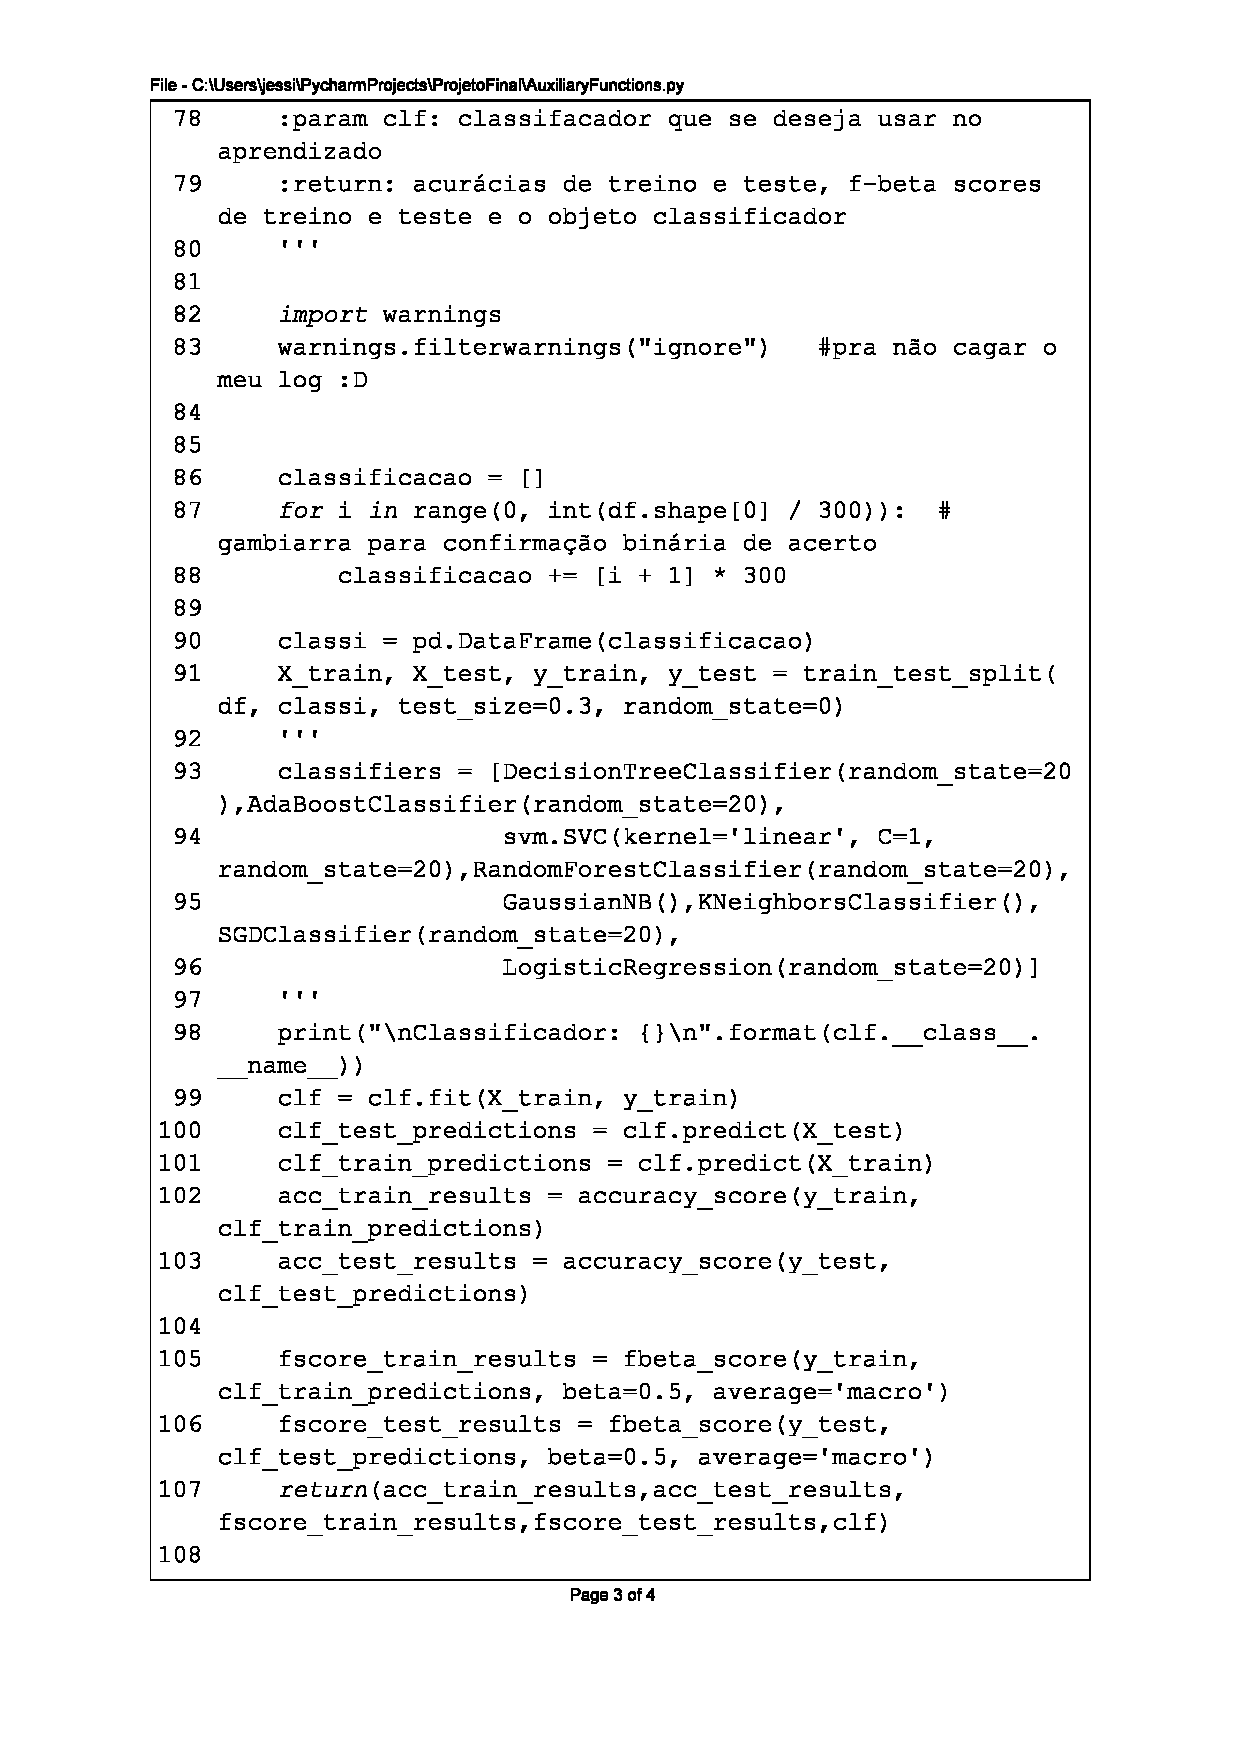
\includegraphics[scale=0.9]{01_Pre_textuais/code/analisa3.pdf}
\end{figure}
\begin{figure}[H]
\centering
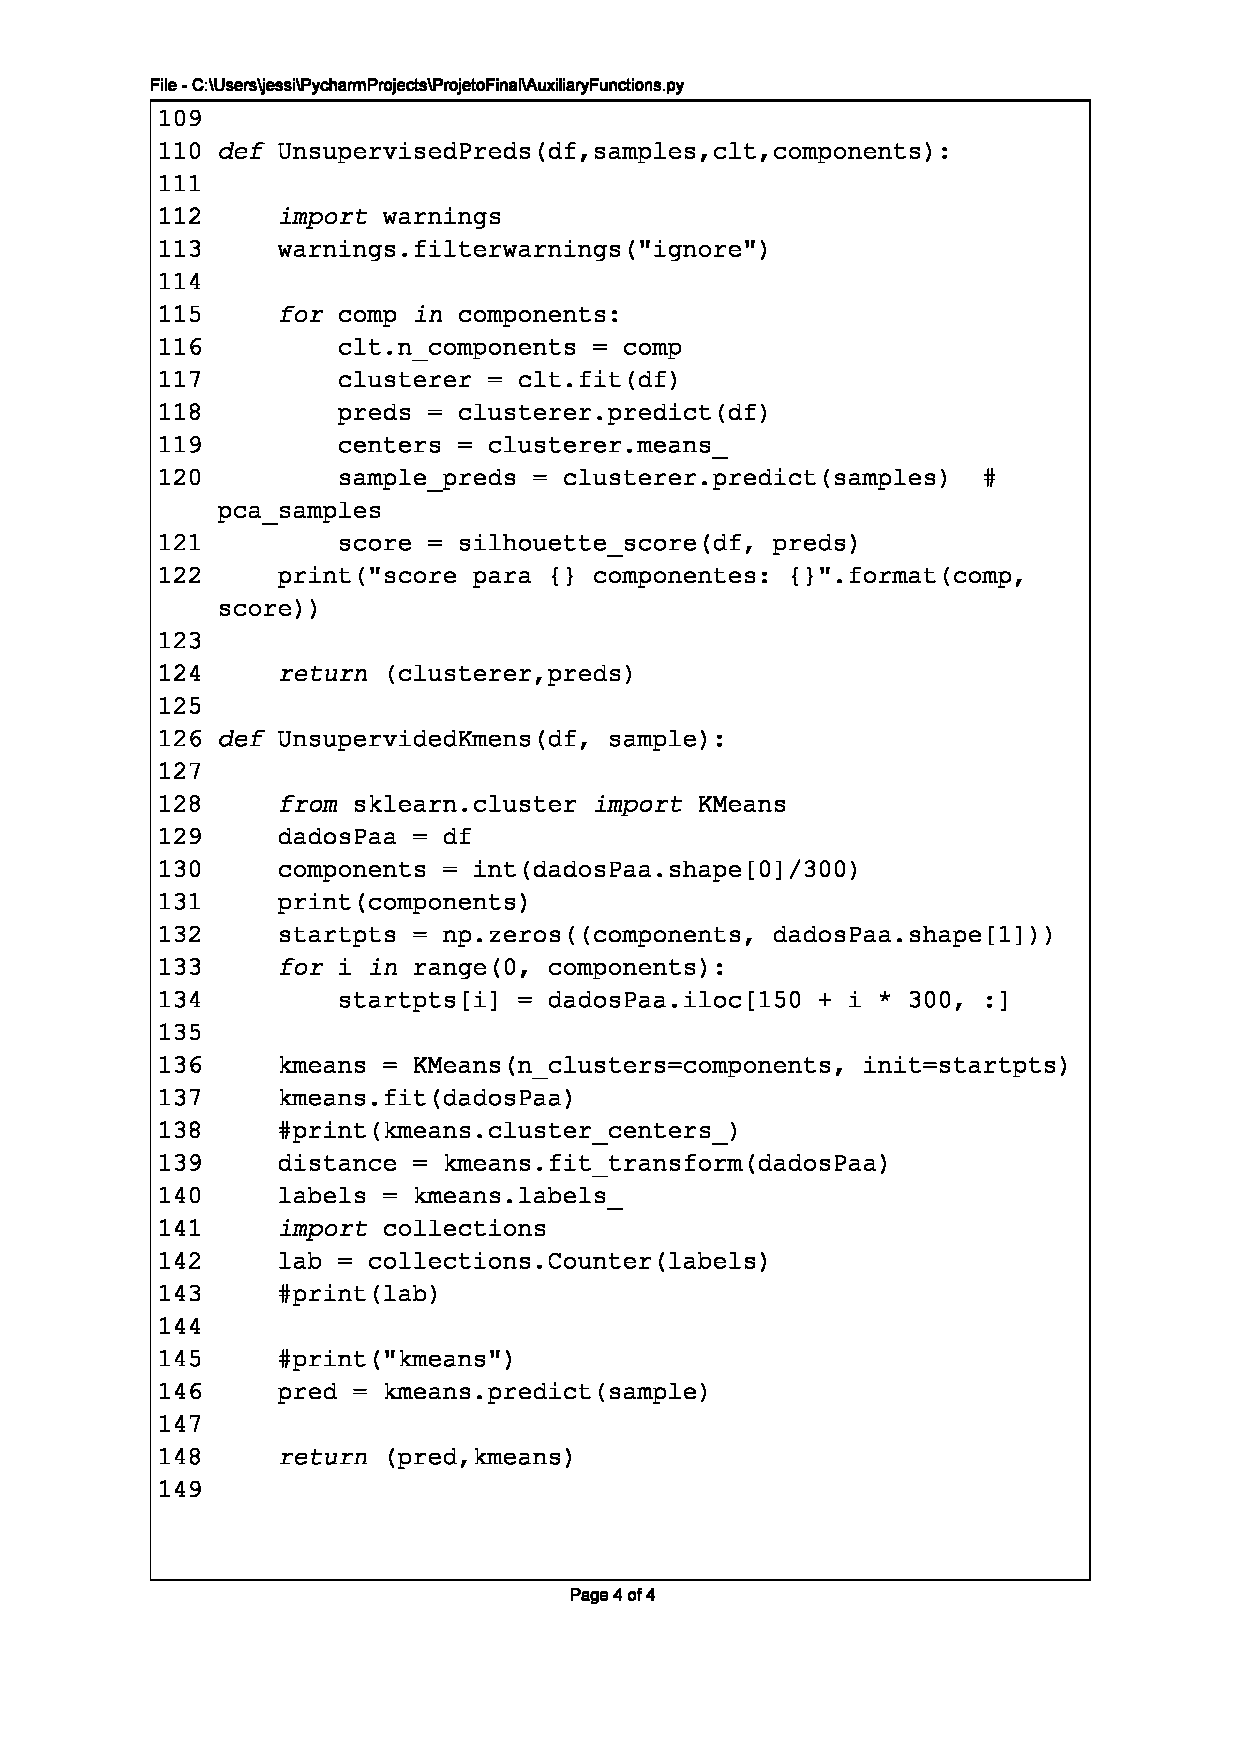
\includegraphics[scale=0.9]{01_Pre_textuais/code/analisa4.pdf}
\end{figure}

 \newpage







\begin{itemize}
    \item Código Principal
\end{itemize}

\begin{figure}[H]
\centering
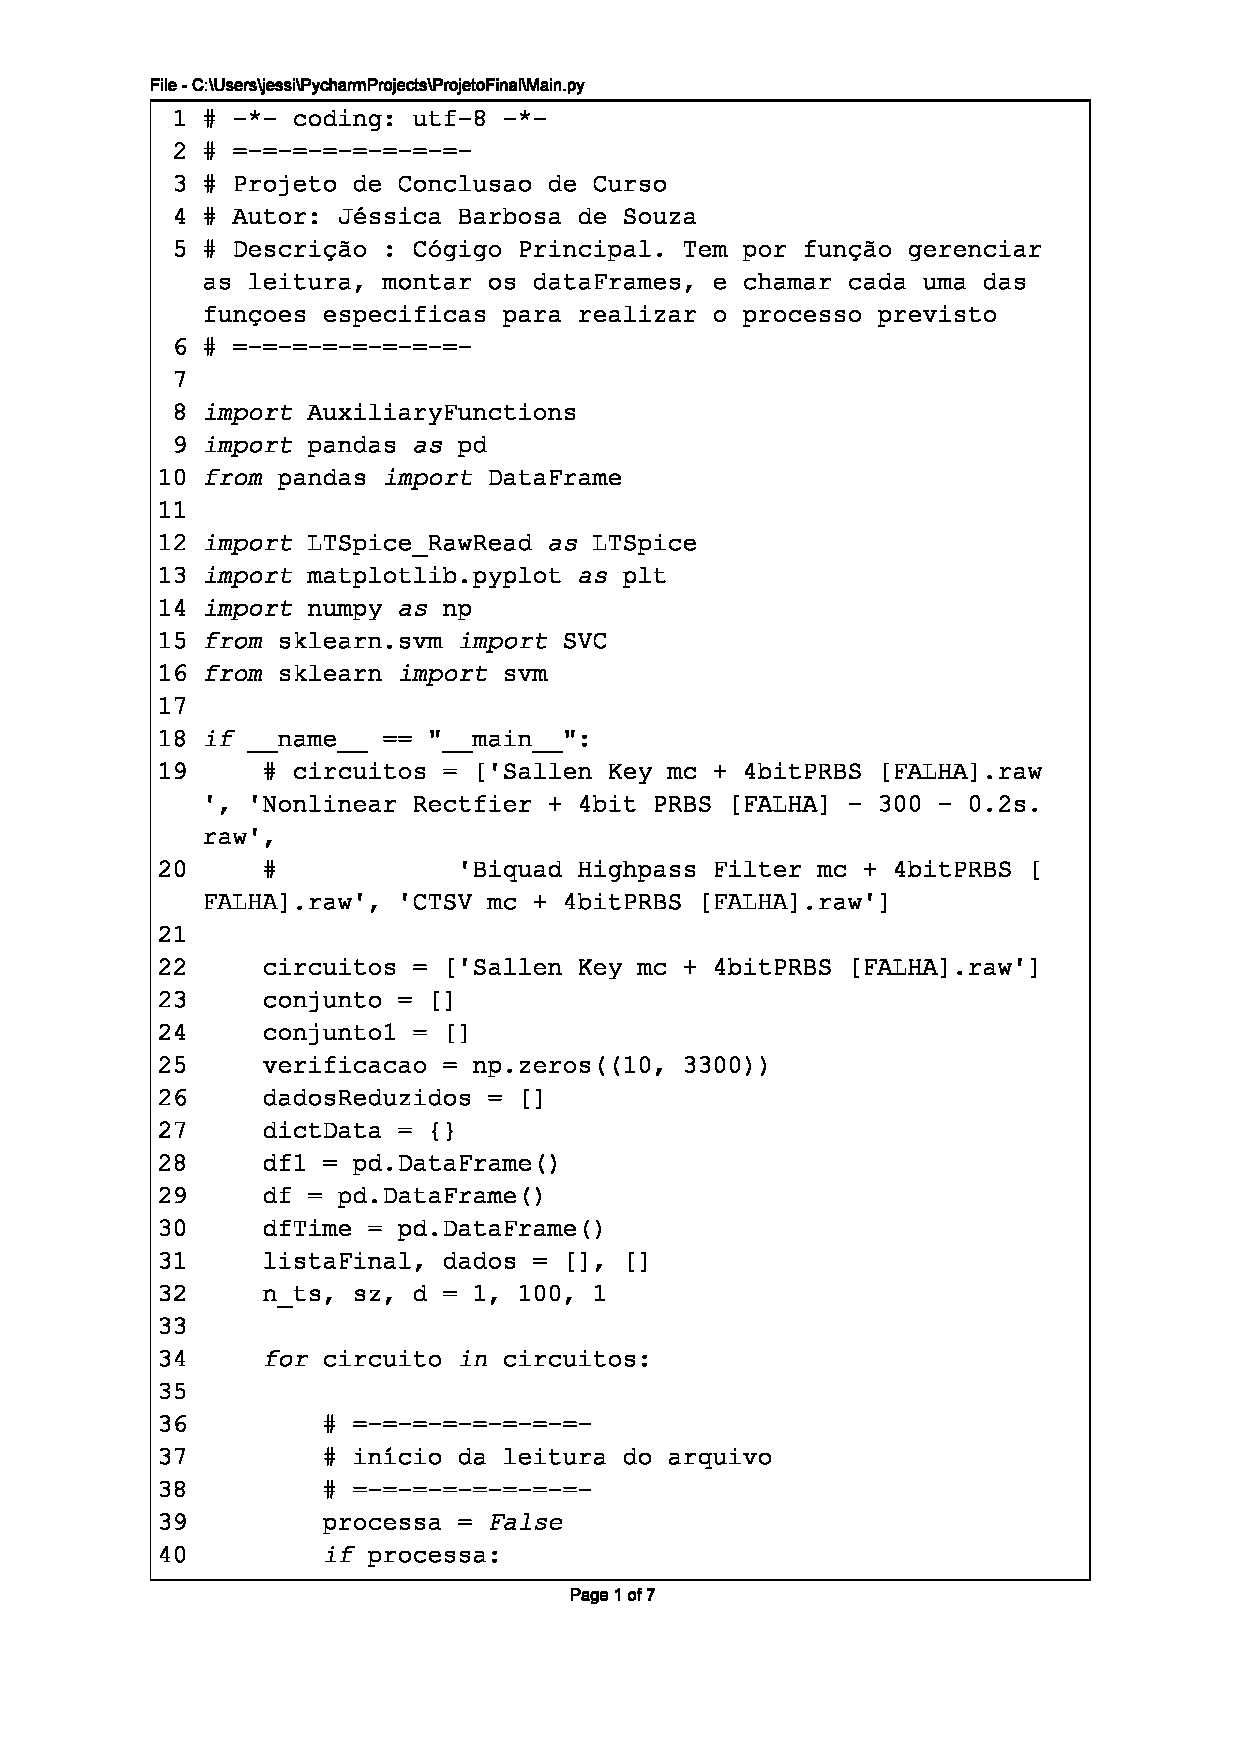
\includegraphics[scale=0.75]{01_Pre_textuais/code/main1.pdf}
\end{figure}

\begin{figure}[H]
\centering
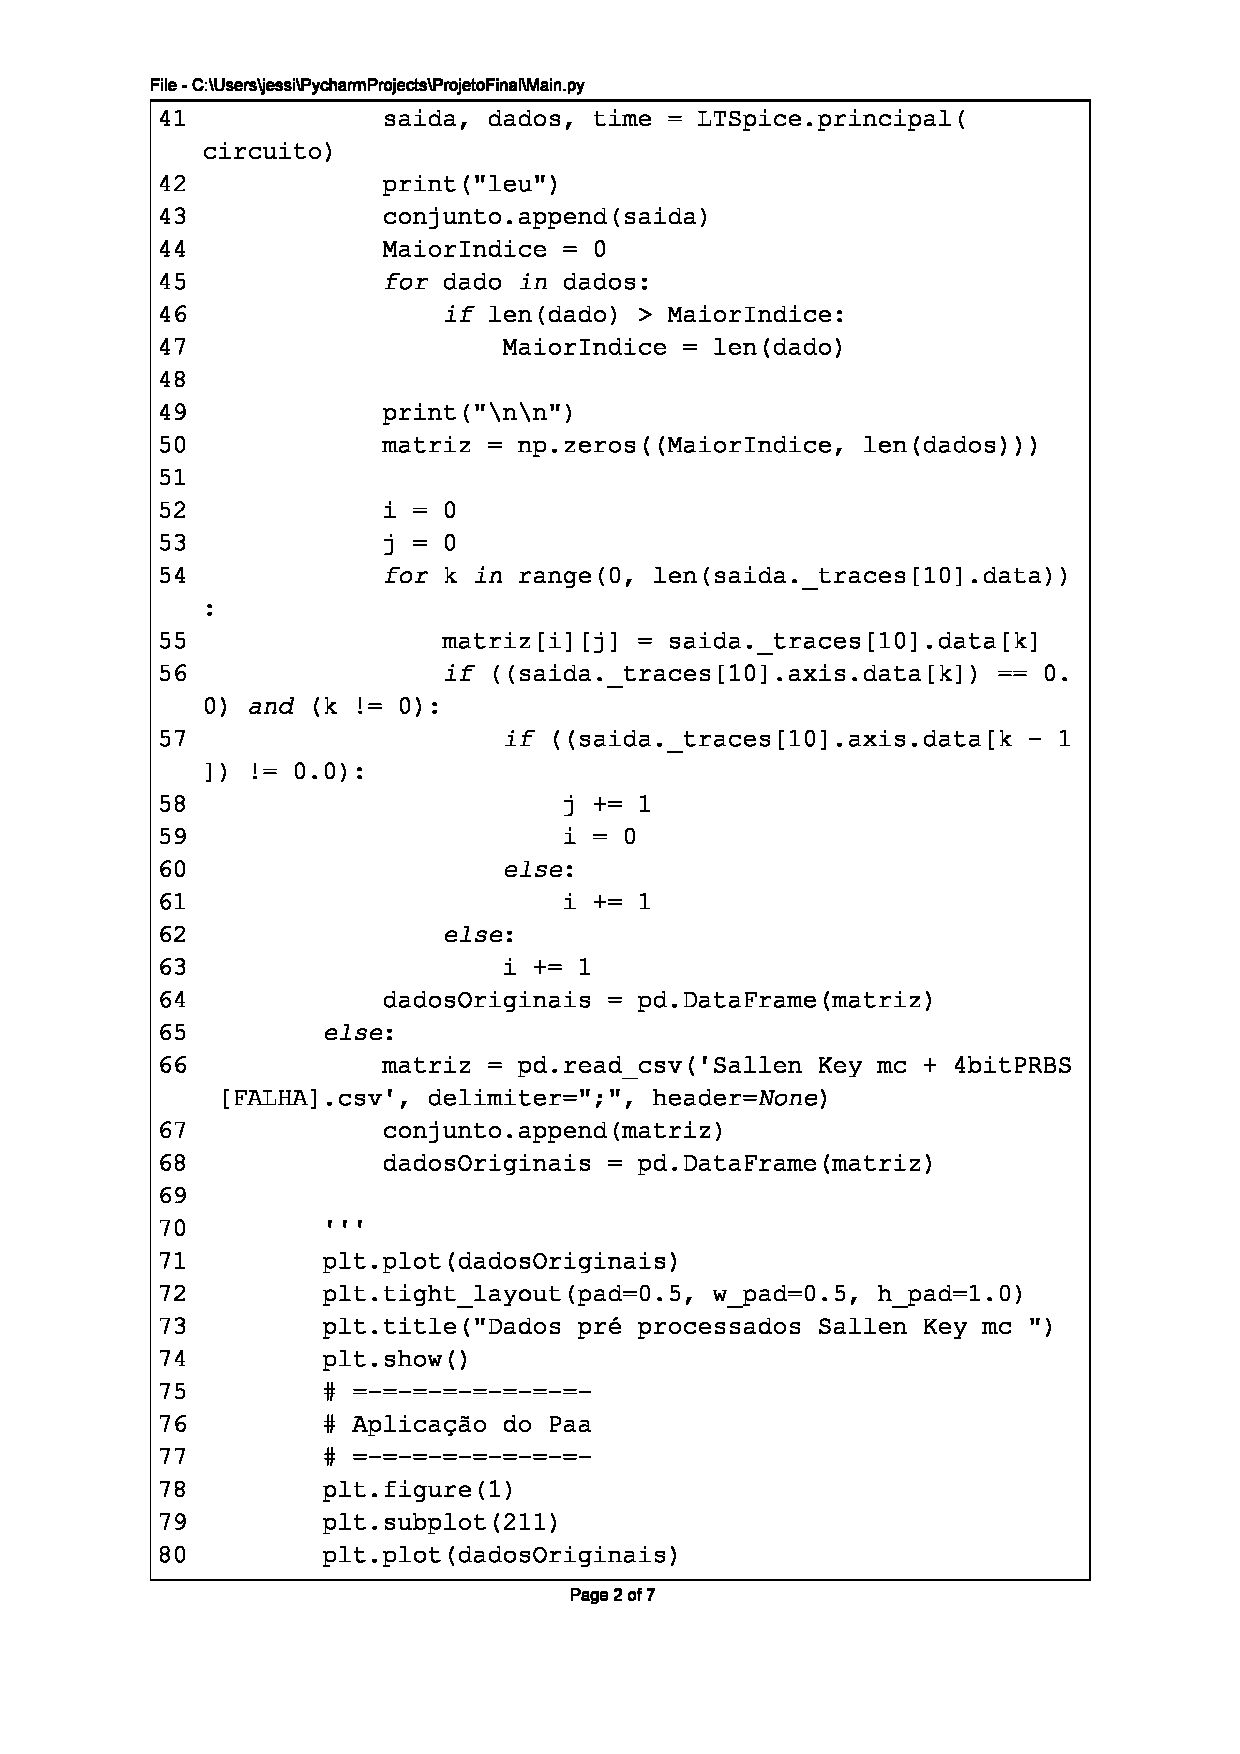
\includegraphics[scale=0.9]{01_Pre_textuais/code/main2.pdf}
\end{figure}
\begin{figure}[H]
\centering
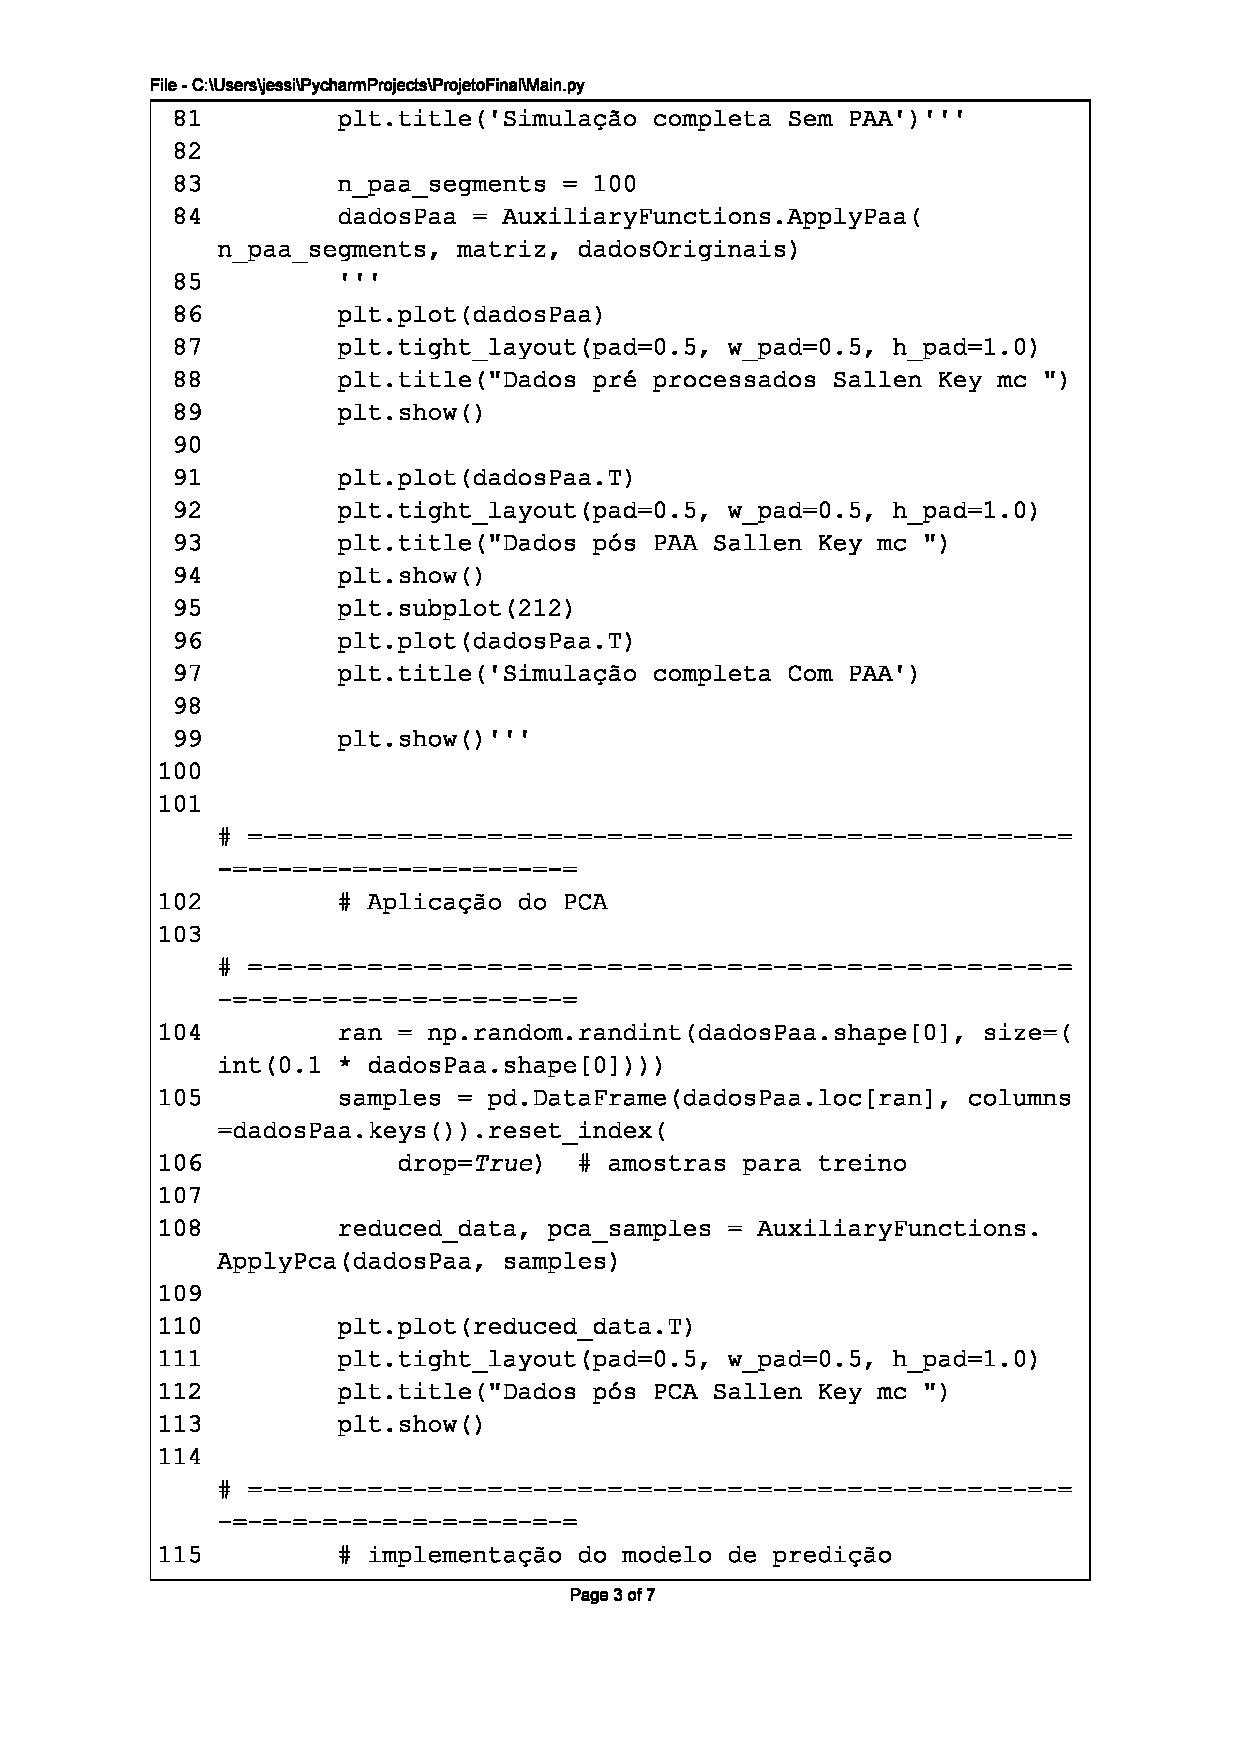
\includegraphics[scale=0.9]{01_Pre_textuais/code/main3.pdf}
\end{figure}
\begin{figure}[H]
\centering
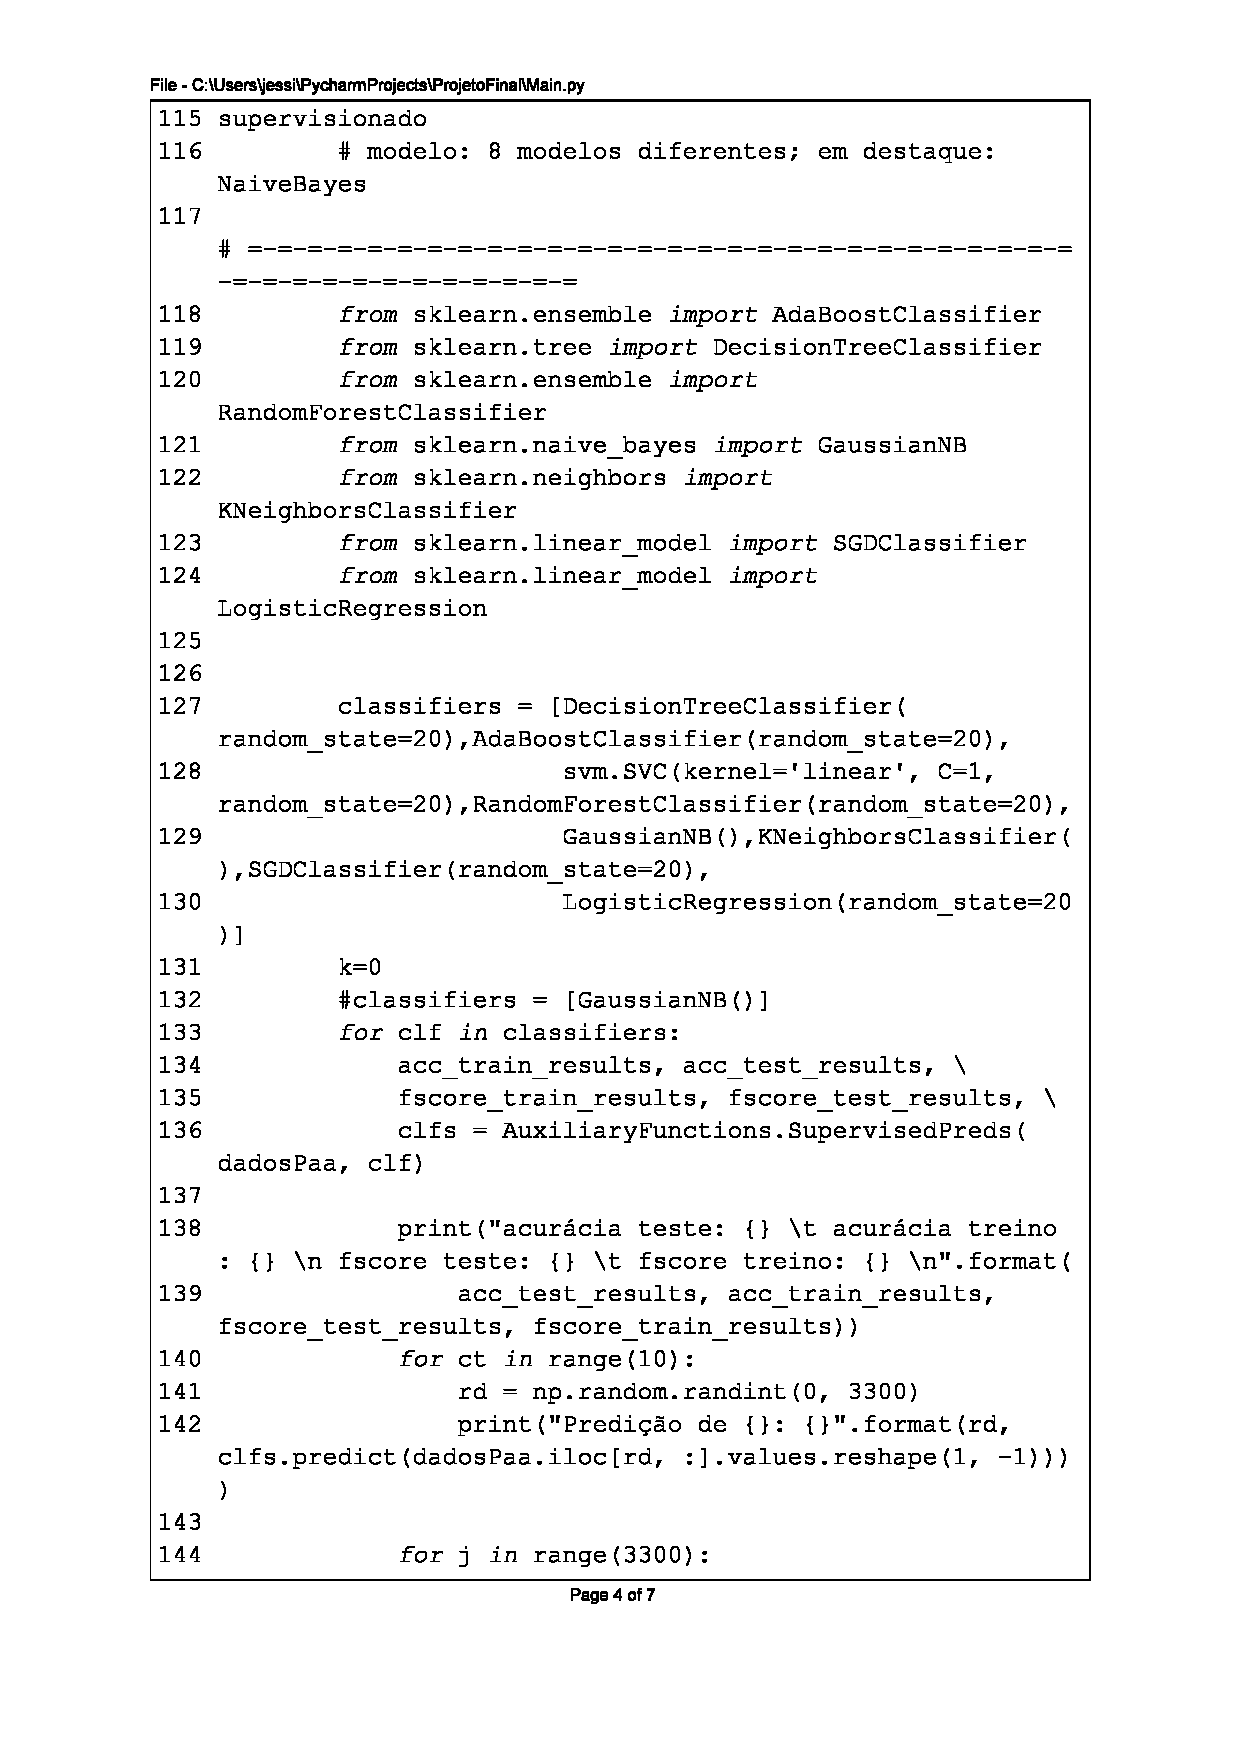
\includegraphics[scale=0.9]{01_Pre_textuais/code/main4.pdf}
\end{figure}
\begin{figure}[H]
\centering
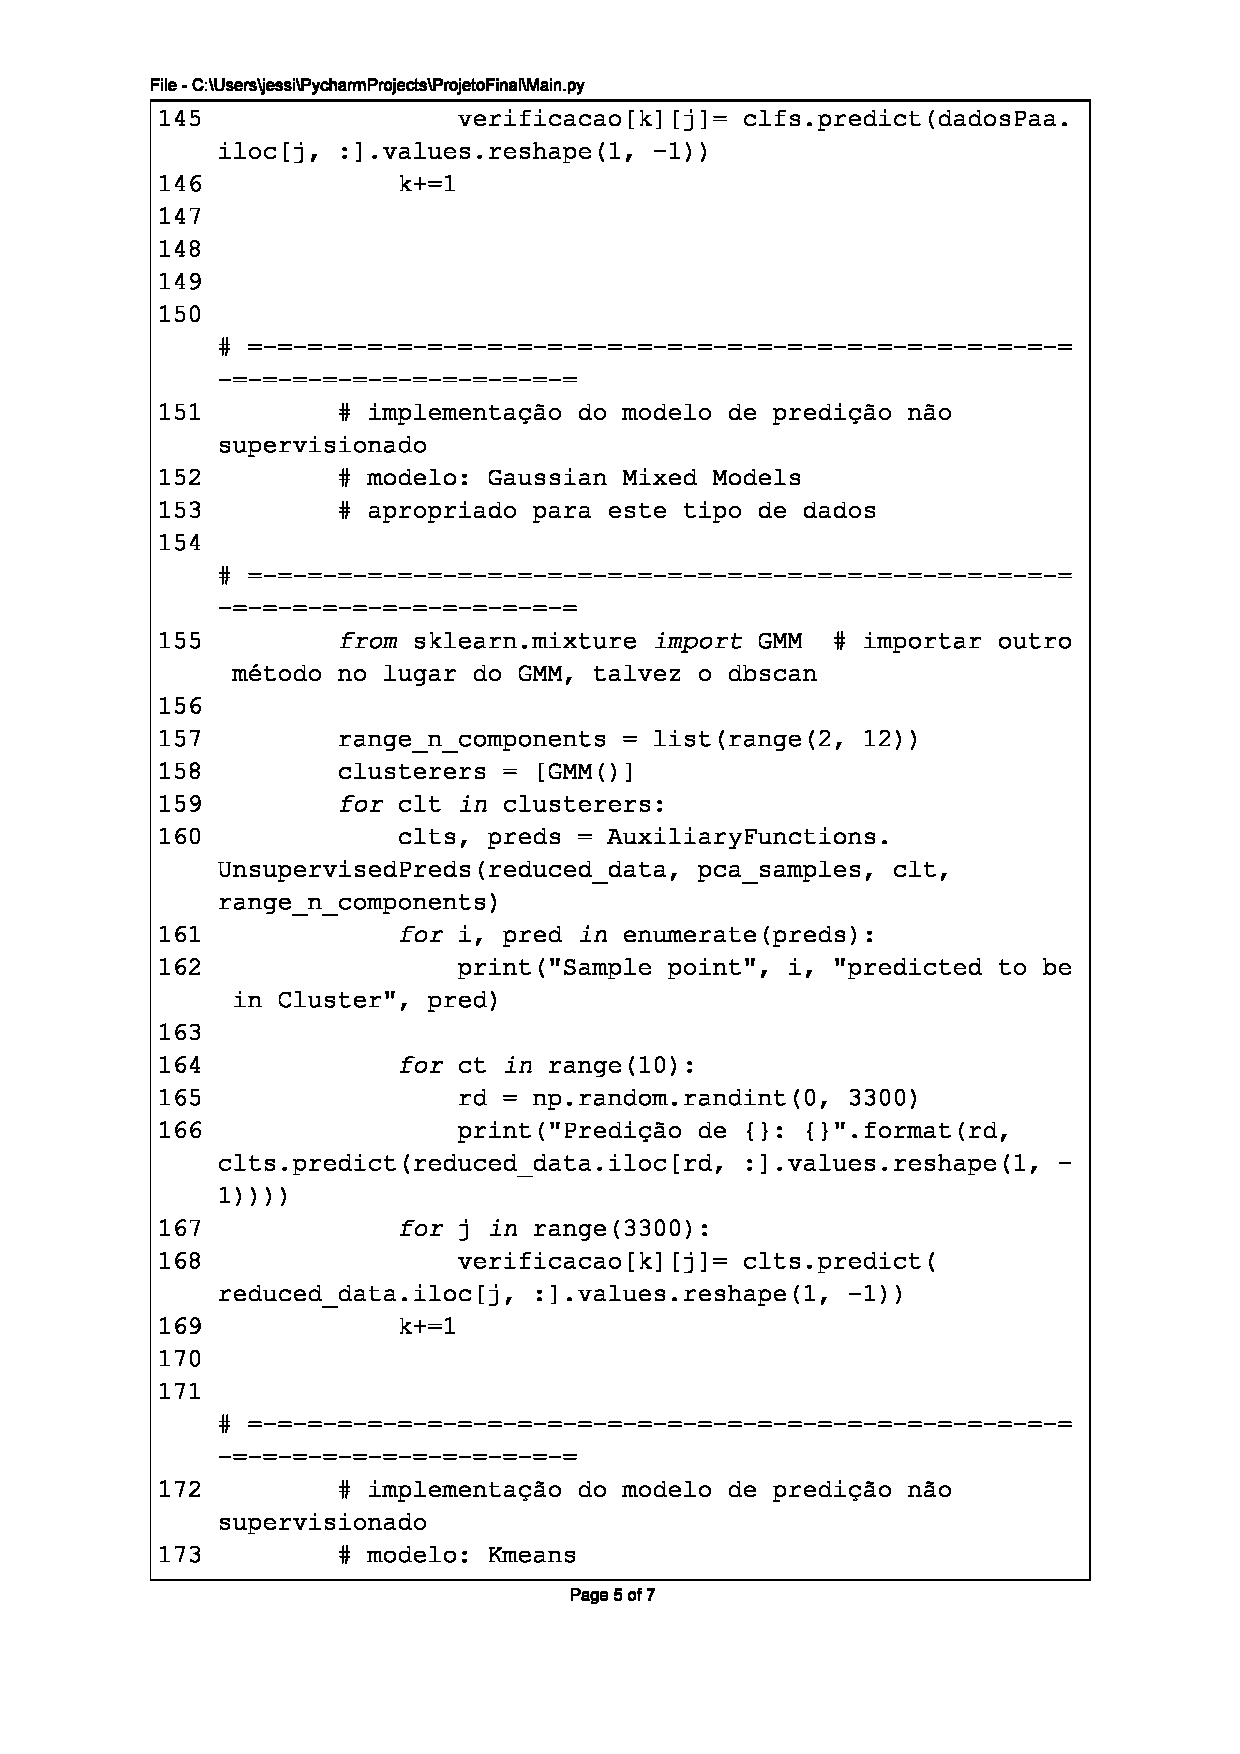
\includegraphics[scale=0.9]{01_Pre_textuais/code/main5.pdf}
\end{figure}
\begin{figure}[H]
\centering
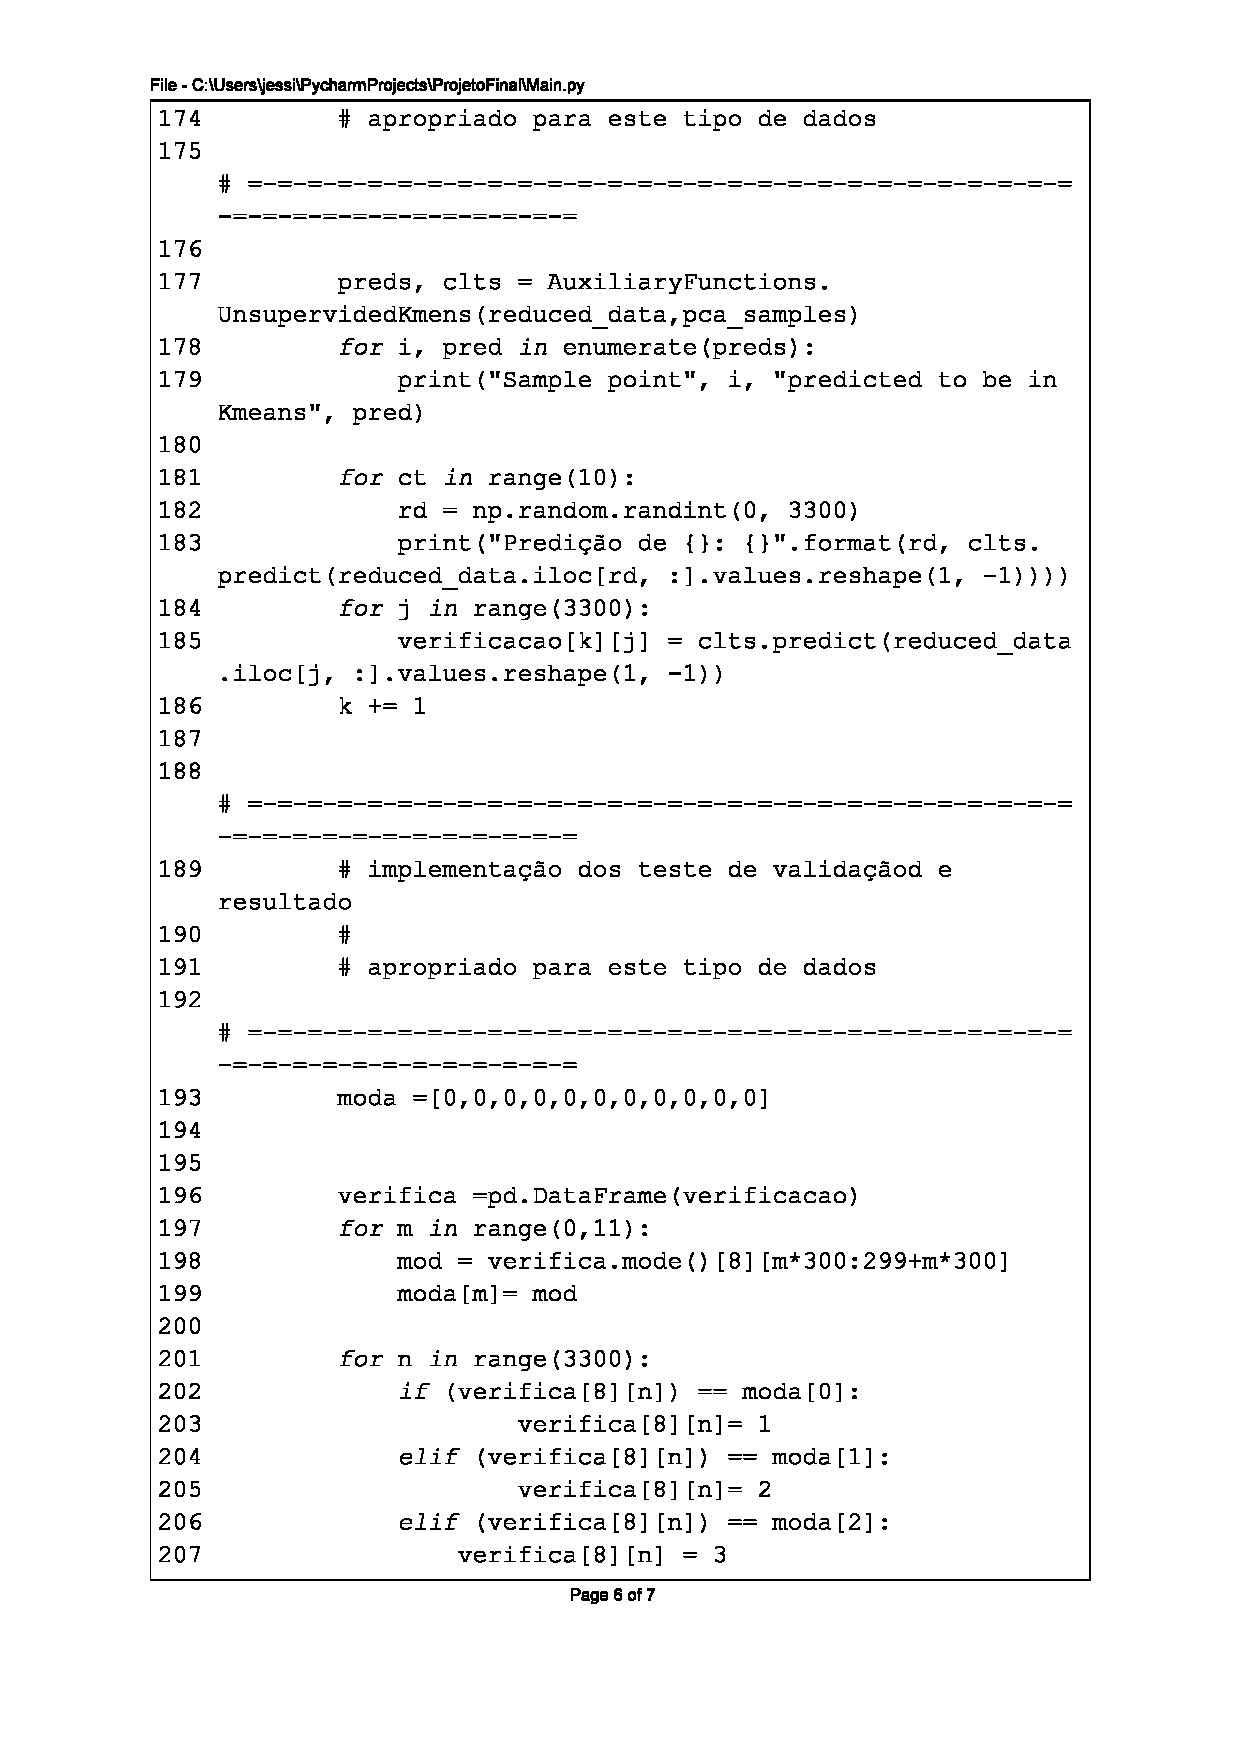
\includegraphics[scale=0.9]{01_Pre_textuais/code/main6.pdf}
\end{figure}
\begin{figure}[H]
\centering
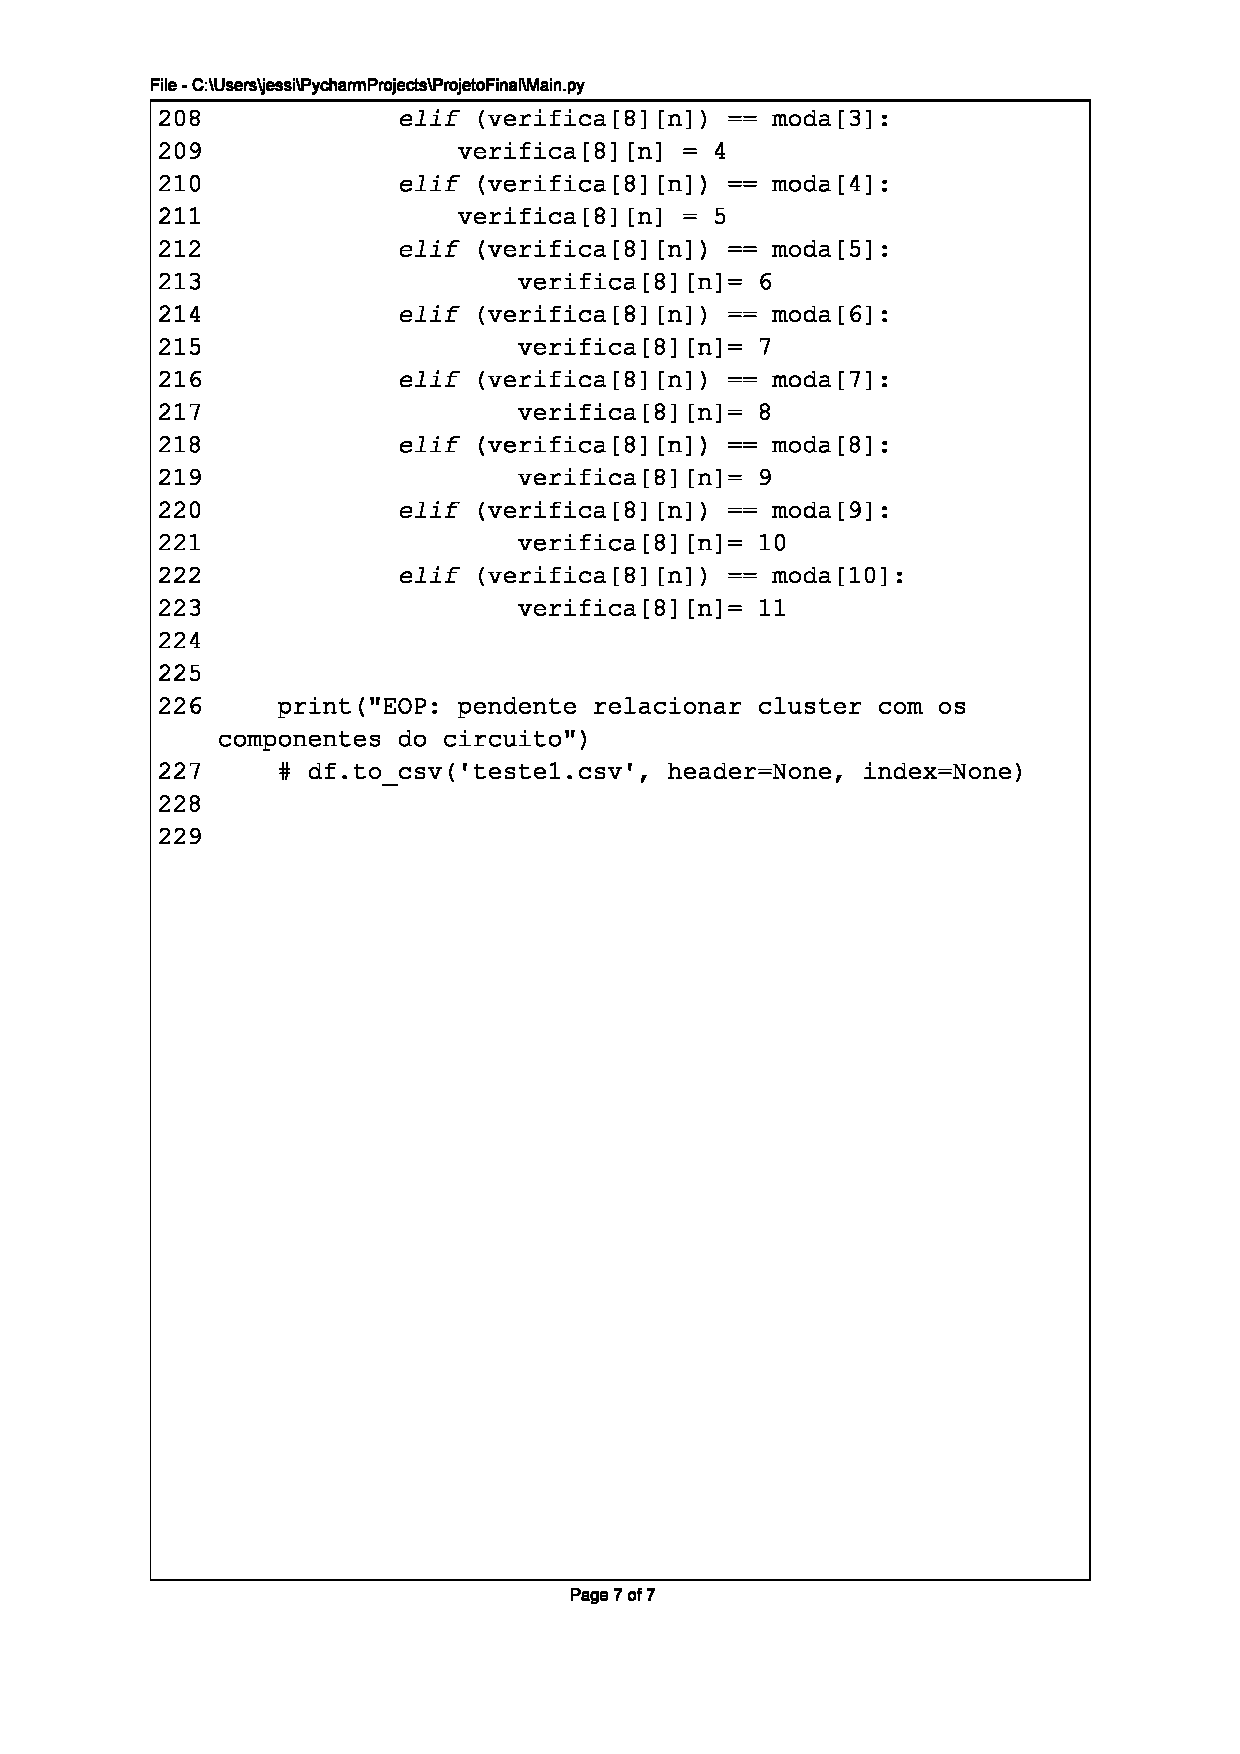
\includegraphics[scale=0.9]{01_Pre_textuais/code/main7.pdf}
\end{figure}



